\documentclass{llncs}

%\pagestyle{plain}
\usepackage{bibnames}
\usepackage{booktabs} % For formal tables
\usepackage{caption}
\usepackage[caption=false]{subfig}
%\usepackage{subcaption}
\usepackage{listings}
\usepackage{xcolor}
\usepackage{graphicx}

\definecolor{mygreen}{rgb}{0,0.6,0}
\definecolor{mygray}{rgb}{0.5,0.5,0.5}
\definecolor{mymauve}{rgb}{0.58,0,0.82}


\newcommand{\myfootnote}[1]{
    \renewcommand{\thefootnote}{}
    \footnotetext{\scriptsize#1}
    \renewcommand{\thefootnote}{\arabic{footnote}}
}

\lstset{ %
  backgroundcolor=\color{white},   % choose the background color; you must add \usepackage{color} or \usepackage{xcolor}
  language=C,
  basicstyle=\scriptsize\ttfamily,
  %basicstyle=\footnotesize,        % the size of the fonts that are used for the code
  breakatwhitespace=false,         % sets if automatic breaks should only happen at whitespace
  breaklines=true,                 % sets automatic line breaking
  captionpos=b,                    % sets the caption-position to bottom
  commentstyle=\color{mygreen},    % comment style
  deletekeywords={...},            % if you want to delete keywords from the given language
  escapeinside={\%*}{*)},          % if you want to add LaTeX within your code
  extendedchars=true,              % lets you use non-ASCII characters; for 8-bits encodings only, does not work with UTF-8
  frame=single,                    % adds a frame around the code
  keepspaces=true,                 % keeps spaces in text, useful for keeping indentation of code (possibly needs columns=flexible)
  keywordstyle=[1]\color{blue},       % keyword style
  keywordstyle=[2]\color{mymauve},       % keyword style
  morekeywords=[2]{*, },            % if you want to add more keywords to the set
  numbers=left,                    % where to put the line-numbers; possible values are (none, left, right)
  numbersep=5pt,                   % how far the line-numbers are from the code
  numberstyle=\tiny\color{mygray}, % the style that is used for the line-numbers
  rulecolor=\color{black},         % if not set, the frame-color may be changed on line-breaks within not-black text (e.g. comments (green here))
  showspaces=false,                % show spaces everywhere adding particular underscores; it overrides 'showstringspaces'
  showstringspaces=false,          % underline spaces within strings only
  showtabs=false,                  % show tabs within strings adding particular underscores
  stepnumber=1,                    % the step between two line-numbers. If it's 1, each line will be numbered
  stringstyle=\color{mymauve},     % string literal style
  tabsize=1,                       % sets default tabsize to 2 spaces
  title=\lstname,                   % show the filename of files included with \lstinputlisting; also try caption instead of title
  xleftmargin=10pt,
}

% Copyright
%\setcopyright{none}
%\setcopyright{acmcopyright}
%\setcopyright{acmlicensed}
%\setcopyright{rightsretained}
%\setcopyright{usgov}
%\setcopyright{usgovmixed}
%\setcopyright{cagov}
%\setcopyright{cagovmixed}

\newcommand{\tanN}[1] {{\color{red}{TanN}}: {\color{red}{#1}}}
\newcommand{\cyC}[1] {{\color{green}{CyC}}: {\color{green}{#1}}}
\newcommand{\johnB}[1] {{\color{blue}{JohnB}}: {\color{blue}{#1}}}
\newcommand{\bryceL}[1] {{\color{cyan}{BryceL}}: {\color{cyan}{#1}}}
\newcommand{\samW}[1] {{\color{violet}{SamW}}: {\color{violet}{#1}}}
\newcommand{\johnS}[1] {{\color{orange}{JohnS}}: {\color{organe}{#1}}}
\newcommand{\daveD}[1] {{\color{purple}{DaveD}}: {\color{purple}{#1}}}

\begin{document}
\title{A DAG-based Programming Tool For Highly Efficient Codes on Accelerators}

\author{
Tan Nguyen,
John Bachan,
Bryce Lelbach,
Samuel Williams,
John Shalf,\\
David Donofrio, and Cy Chan}
\institute{Lawrence Berkeley National Laboratory, USA\myfootnote{Email: tannguyen@lbl.gov. Bryce Lelbach recently moved to NVIDIA.}
}

\maketitle

\begin{abstract}
Recently, heterogeneous architectures have gained traction in HPC. 
Systems with deep and complex hardware hierarchy and equipped with accelerators each having thousands of cores are increasingly commonplace. 
Optimizing application codes for scalability on such hardware design is extremely challenging, since it requires effective management of the massive thread pool and the ability to balance the workload and hide communication cost among threads/accelerators.
To alleviate these labor intensive jobs, we present a solution based on task parallelism, abstracting away many hardware details associated with sophisticated accelerator architectures such as GPUs. 
We also develop a runtime system called RambutanAcc that can schedule coarse and fine-grain tasks on NVIDIA's GPUs.
Using two HPC benchmarks, we demonstrate the effectiveness of our tool without intrusively modifying the source code.
\end{abstract}


\section{Introduction}
\label{sec:intro}
It is very likely that exascale systems will be armed with powerful accelerators and/or many-core processors.%~\cite{ASCRExascaleLethin, exascaleRoadMap}. 
On such systems, performance will heavily depend on how compute kernels harness each accelerator or many-core processor, which often requires aggressive, low-level kernel optimizations that destroy portability across systems with different processor architectures.
Specifically, the programmer must perform different sets of potential optimizations on the same compute kernel for different architectures.
This problem is challenging especially for domain programmers, given that they must also optimize the communication among multiple accelerators within each compute node as well as across nodes.

This paper presents a solution that allows the programmer to explore effective optimizations for an application on a given hardware without aggressive modifications to the source code. 
Specifically, we exploit task-based parallelism that can abstract away complicated hardware details associated with low-level accelerator architectures.
%We extend the programming interface of {\em Rambutan}~\cite{rambutanWebsite}, which 
We provide an interface to construct dynamic task dependency graphs that unfold as the program executes. 
Tasks can execute as soon as their {\em true} data dependencies are satisfied, thus avoiding many types of over-synchronization (e.g. barrier, wait\_all, etc.) present in traditional programming models.

We also develop a task-based runtime that can dynamically schedule both coarse and fine-grain tasks.
Each task of the input graph can be scheduled to run on a {\em worker}, which can be either a group of CPU cores, an accelerator, or a group of accelerator cores.
%\cyC{"group of accelerator cores" would be clearer than "a partition of an accelerator", which hasn't been defined yet}
Our runtime handles communication among tasks automatically -- in particular, data required by a task can be produced by other tasks running anywhere else on the system.
%, i.e. on a CPU or accelerator on a local or remote compute node.
%The programmer has a choice to select the communication path, 
The runtime then transparently moves data to where the dependent task will execute, and handles communication in the background so that communication can be overlapped with computation of other runnable tasks.
%\sout{Not only can data move, but tasks can also migrate among different memory address spaces via work stealing.
%Specifically idle workers can find chance to steal tasks from other workers, enabling dynamic load balancing}.
Dependent data can either be routed through the host or moved directly between accelerators when hardware support is available.
%\cyC{why not utilize direct device to device transfer when the hardware is available?  what is the benefit from giving the programmer a choice?}

%{\em RambutanAcc} 
Our runtime currently supports NVIDIA's GPUs.%and the first generation of Intel's Xeon Phi co-processor (KNC).
%In this paper, we present the GPU supported version as the GPU code (e.g. CUDA) is substantially different from conventional code running on the CPU.
With a simple programming model, it removes the programming burden of launching CUDA kernels and moving data between the host and GPUs.
Each task can be specified as a conventional routine parallelized across a thread team.
%In typical CUDA code, running multiple types of tasks requires launching multiple independent kernels, with little flexibility in when tasks of different types may be executed.
%In contrast, 
%{\em RambutanAcc} 
The runtime can be configured to launch a single {\em persistent CUDA kernel} that can service multiple requests from a task scheduler running on the host, thus avoiding the overhead of multiple kernel launches during execution.
The persistent kernel partitions available streaming multiprocessors (SMs) of a GPU into separate workers, each of which have the flexibility to asynchronously service tasks of different types, increasing task parallelism.
%This method provides much more flexibility to overlap communication with useful computational work.
%{\em RambutanAcc} 
The runtime is also equipped with a communication handler to service data transfer requests across GPUs and between the host and GPUs.
This handler utilizes CUDA streams and works asynchronously with the persistent kernel.
The handler can also move data directly among the GPUs via direct memory access (DMA).
%\footnote{For MIC-based workers, we use Intel's COI (co-processor offload infrastructure) to implement the on-node handler.}
%For off-node requests, we use GASNet~\cite{Bonachea:2002:gasnet}, a one-sided communication library % , to implement the communication handler.
that provides non-blocking data transfer and low-latency signaling mechanisms. % , allowing inter-process communication to be overlapped with computations efficiently.

We evaluate our tool with two HPC benchmarks: sparse Cholesky factorization and a 3D stencil solver for Laplace's equation.
%\samW{needs to be consistent with sec5... missing ML code}
The results show that the performance improves significantly and meets the performance level of our painstakingly hand-optimized code variants.
%{\em RambutanAcc} also hides communication costs that cannot be avoided.\samW{how is this different than the previous sentence?}
In addition, for sparse cholesky factorization, having multiple workers on a single GPU allows compute throughput to be increased at low programming cost. 
We hope this result will encourage further research to develop and tune sparse kernels for co-scheduling fine-grained tasks on GPUs.
%The contributions of the paper are three-fold.
%\begin{itemize}
%\item A task-based programming model that can reveal a significant amount of dynamic parallelism in an application
%\item A runtime system that supports a rich set of task scheduling and communication handling policies for learning the impact of various optimizations on the performance
%\item A thorough experimental study using four HPC benchmarks 
%\end{itemize}
Our original contributions are as follows:
\vspace{-0mm}
\begin{enumerate}
	\item We present a DAG-based programming model that provides a portable programming abstraction layer to enable high performance on accelerated HPC architectures.
	\item We present an asynchronous execution model that provides optimization of fine-grained task scheduling on accelerators (with multiple independent workers per accelerator) and automatic communication-computation overlap between tasks.
	\item We demonstrate the effectiveness of using a persistent accelerator kernel in the context of a fine-grained task based scheduling.
	\item We show the benefit of utilizing direct accelerator-to-accelerator communication hardware support in the context of a task-based programming and execution model.
\end{enumerate}

The rest of this paper is organized as follows.
Sec.~\ref{sec:motivation} presents the overview of a hybrid system, which is increasingly popular in practice.
In Sec.~\ref{sec:model}, we present the task-based programming model.
Followed by this section is Sec.~\ref{sec:impl}, which discusses the implementation of the associated runtime.
Sec.~\ref{sec:results} shows experimental results.
Sec.~\ref{sec:related} presents related work.
We conclude the paper in Sec.~\ref{sec:conclusion}.


\section{Heterogeneous Node - a Notable Design Trend}
\label{sec:motivation}
Looking at system designs towards Exascale~\cite{top500}, one will not hesitate to predict that future systems will be based on more powerful compute nodes rather than more nodes~\cite{Shalf:exascaleChallenges}.  
An inevitable consequence of this design trend is that node architecture will be more complex.
Indeed, it is common to see traditional multi-core CPUs augmented with multiple high-end graphics cards such as NVIDIA's GPUs.
Other accelerator architectures such as FPGA~\cite{Chen:Eyeriss}, Automata Processor \cite{Fang:UAP}, and Neuromorphic Processor \cite{kim:neuromorphic} have also been gaining more traction.
Heterogeneous programming is challenging~\cite{exascaleRoadMap}, mainly because realizing high performance and scalability on accelerators is difficult.
Even when an application performs well on accelerators, load imbalance arises since CPUs and accelerators run at different rates.
Beside the problems above, the programmer has to handle the communication between CPUs and accelerators, e.g. via PCIe, NVLink, etc.
% (see Fig.~\ref{fig:sysArch}).
In this paper, we focus on tackling challenges associated with the heterogeneous CPU-GPU node design, though our solution can also support the homogeneous case and be extended to support other accelerator architectures.

%To avoid these problems, compute nodes can be based on stand-alone many-core processors such as the Intel's second generation Xeon Phi processor (KNL).
%However, applications consisting of both task and data parallelism may not be well-suited to such homogeneous designs.
%In addition, realizing expected performance on stand-alone many-core processors also requires expert programming skills
%to manually manage data movement and locality.

%\begin{figure}[htb]
%\centering
%\begin{subfigure}[b]{0.22\textwidth}
%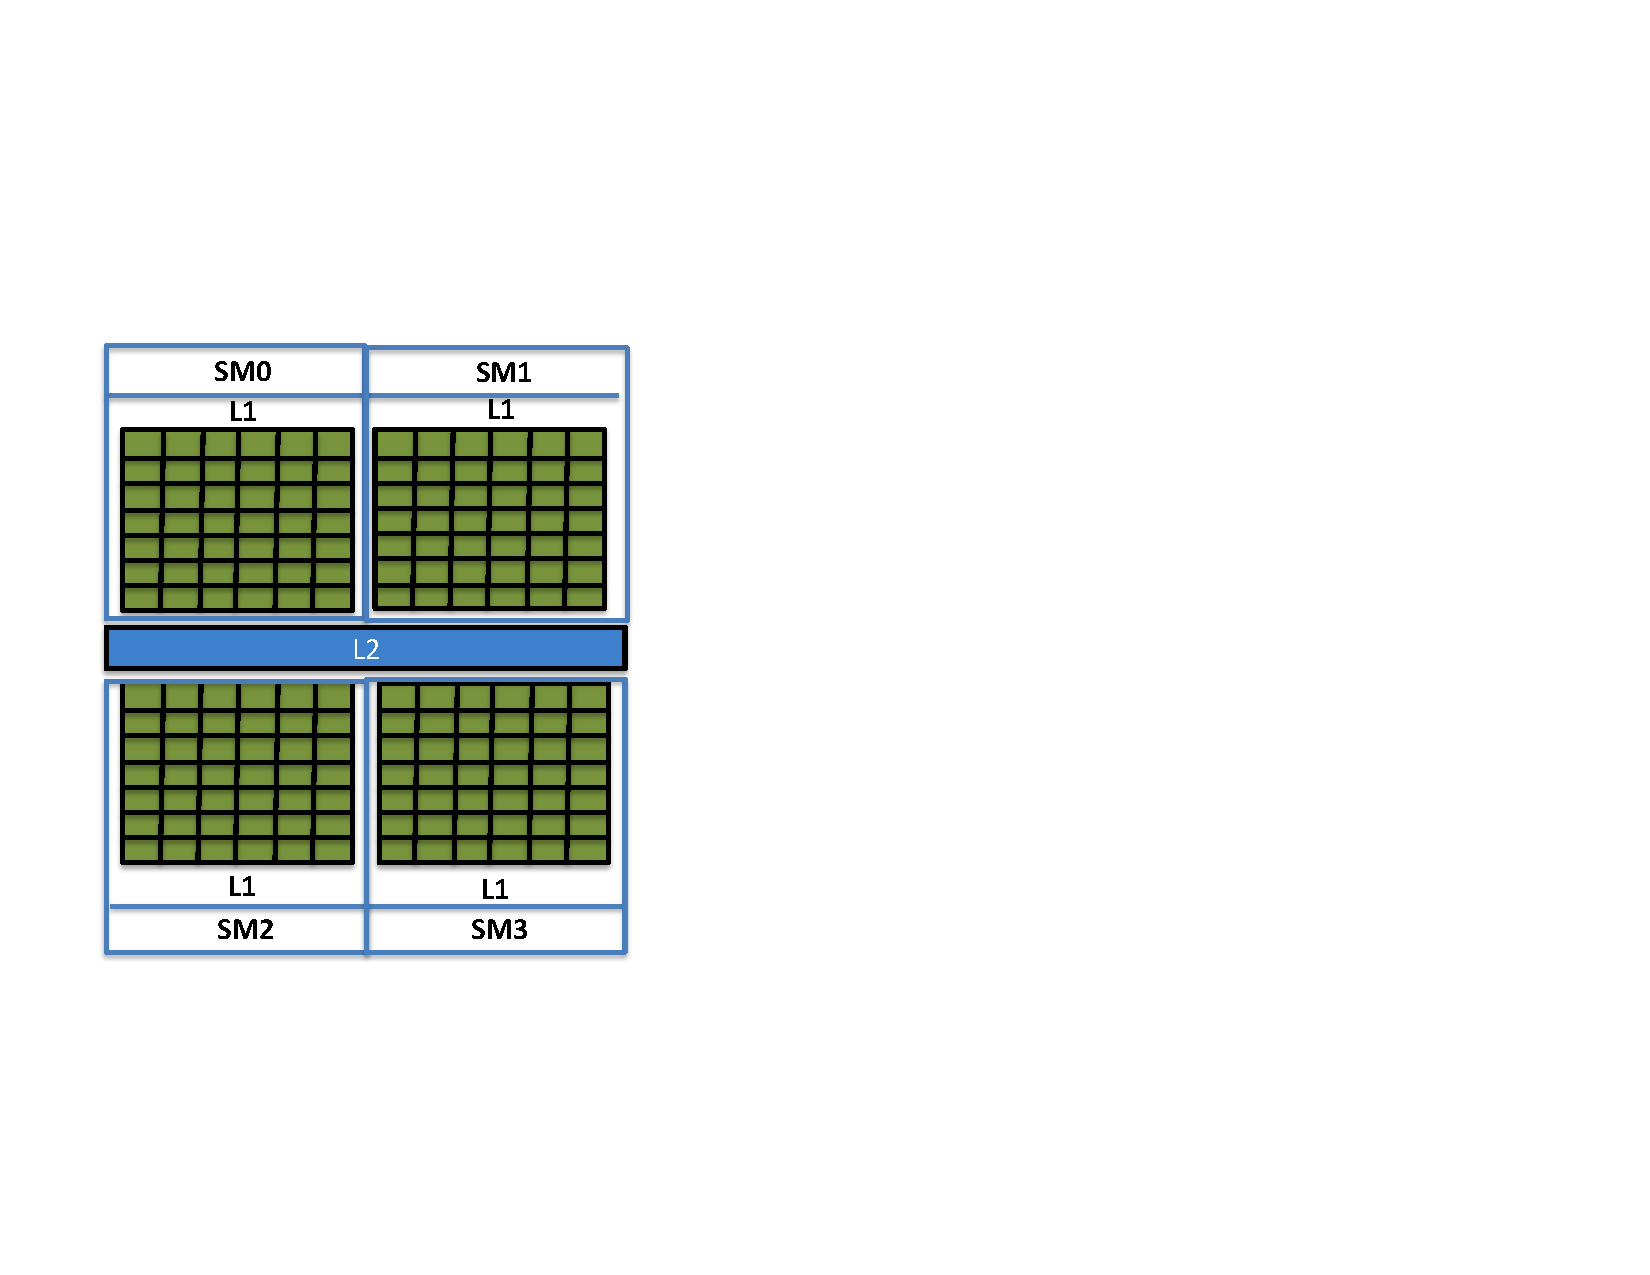
\includegraphics[width=\textwidth]{figures/SMs.pdf}
%\caption{A GPUs with 4 SMs}
%\label{SMs}
%\end{subfigure}
%\begin{subfigure}[b]{0.2\textwidth}
%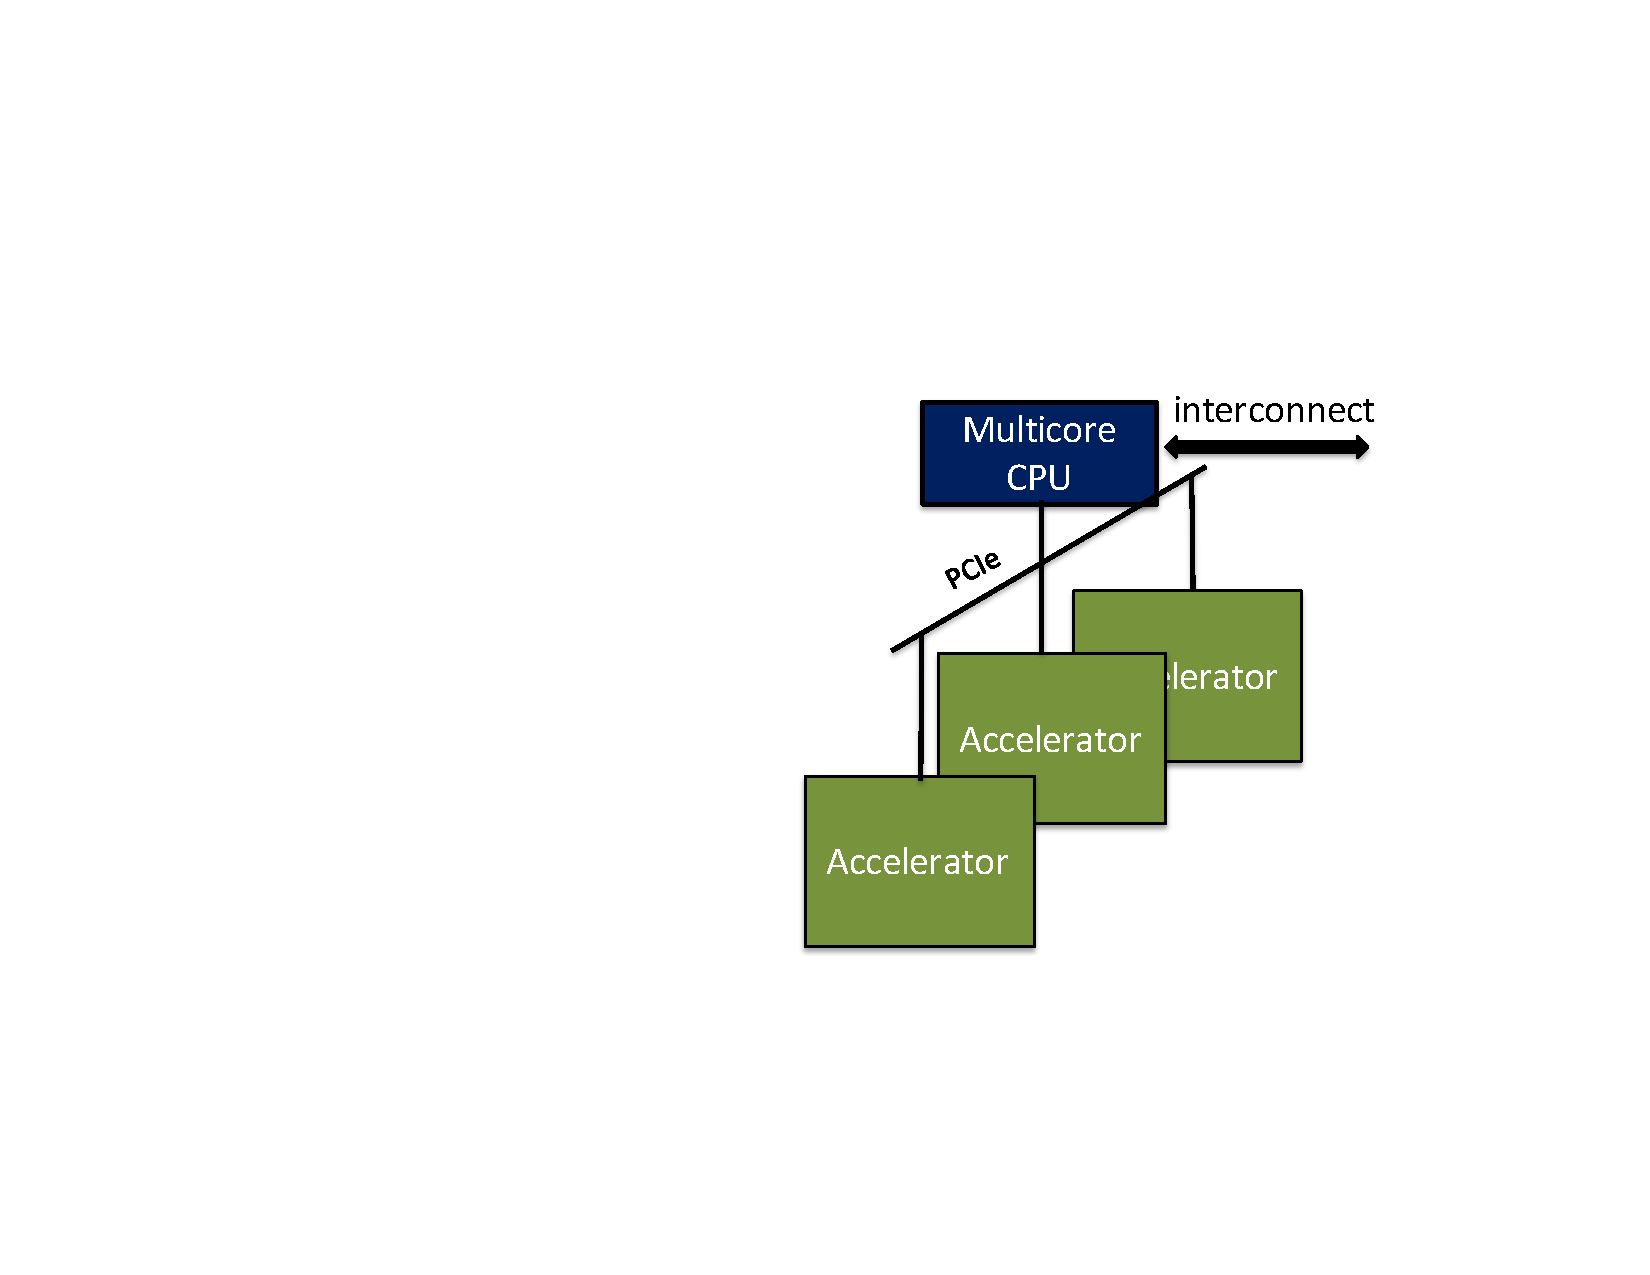
\includegraphics[width=\textwidth]{figures/host_accelerator.pdf}
%\caption{Host with accelerators}
%\label{hybrid}
%\end{subfigure}
%\caption{A hybrid node design}
%\label{fig:sysArch}
%\end{figure}




\section{Programming Model}
\label{sec:model}
In this section, we present a task dependency graph programming model and its associated execution model.
Our design goal is to keep the programming API as simple as possible.


\subsection{Task and Data Spaces}
At the high level, an application can be represented by a directed acyclic graph (DAG) in which vertices are {\em tasks} (see Fig.~\ref{fig:cholesky}),
and edges are data or control {\em dependencies}.
Our programming interface defines {\em task spaces} and {\em data spaces}.
A task space encapsulates the behavior of a class of tasks.
A task is an atomic sequence of statements, in the sense that when a task is scheduled it runs to completion.
Tasks are created and destroyed dynamically at runtime, so only the active portion of the task graph must reside in memory.
A data space encapsulates access and management of a class of data.
%\cyC{Prefer not to use the term "data partition"}
% The programmer specifies task inputs and outputs, which are data partitions.
The programmer specifies task inputs and outputs, which are called data {\em parcels}.
Each parcel is associated with an attribute called a {\em locale}, which indicates the location of the parcel (e.g. in GPU's memory).
% The programmer defines an ownership function to map tasks to partitions of the data space.
The programmer also defines an ownership function to map tasks to locales.
If a parcel a task requires does not reside in the same locale, the runtime will automatically transfer it.
We next describe the full process of defining a task.

\begin{figure}[htb]
\centering
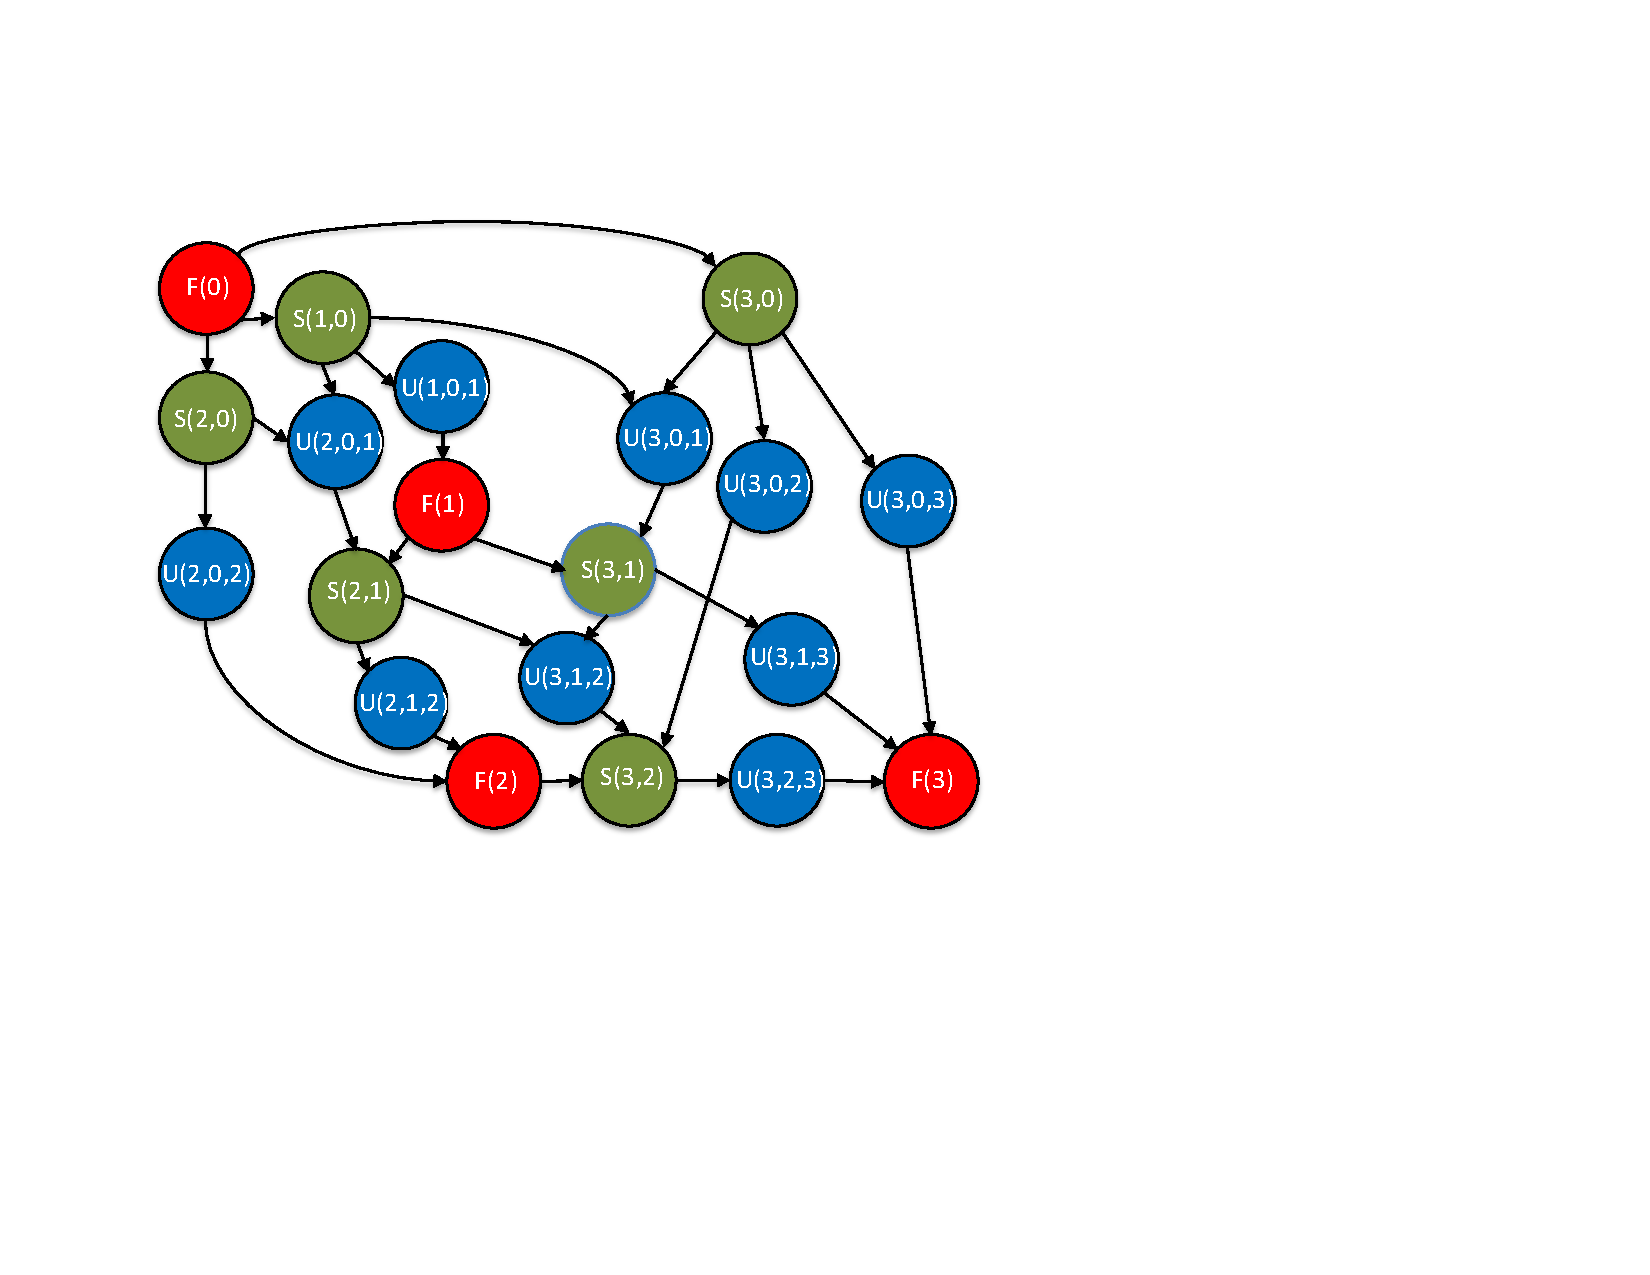
\includegraphics[width=.6\textwidth]{figures/cholesky.pdf}
\caption{Cholesky factorization DAG consisting of three types of tasks: F (Factor), S (Solve), U (update). Each task is associated with a partition of the input matrix called a {\em tile}. Arrows presesent data dependencies between tasks of different types or of the same task type but on different tiles. All data dependencies are called parcels.}
\label{fig:cholesky}
\end{figure}



\subsection{Defining a task}
\label{sec:task-def}
We support 3 types of task: (1) tasks running completely on the host, (2) tasks running on a group of accelerator cores, and (3) tasks running on host and offload kernels to the accelerator that comes along with host.
The first type supports computation on conventional processors (e.g. Intel's Ivy Bridge, AMD's Opteron, IBM's Power 8)  and many-core processors such as Intel's KNL.
The second type is for studying the benefit of fine-grained scheduling on a group of accelerator cores such as GPU's SM (Symmetric Multiprocessor), whereas the third type is useful when the programmer needs to retain legacy kernel code and study the communication among accelerators.
In the Cholesky factorization graph in Fig.~\ref{fig:cholesky}, it is reasonable to define {\em Factor} and {\em Solve} with the first type since they have low compute intensity. 
{\em Update}, on the contrary, should be defined to run on a group of accelerator cores (type 2) or on the whole accelerator (type 3).

For tasks running completely on the host (type 1), the process of defining a task includes the specification of data inputs and outputs, statements that the task will execute, and actions that should be performed upon completion of the task (e.g. create new tasks).
Defining inputs, outputs, and the post-completion action for tasks of type 2 and 3 are similar to type 1; however, the execution code for these two types is slightly different.
Specifically, the task code must be multithreaded and the abstract thread hierarchy for these tasks is very deep to support a substantially larger number of cores.
Fig.~\ref{fig:program} shows the kernel code of the {\em Update} task of sparse Cholesky factorization, which is a sparse-sparse matrix multiply operation.
Like the CUDA programming model, each task kernel is executed by many threads (called a thread grid), organized into SIMD teams, each scheduled to run on a group of cores.
Teams scheduled (normally in a pipelined fashion) on the same group of cores are called thread blocks.
Type 3 tasks will invoke this kernel using a kernel launch interface (defined by hardware vendor such as NVIDIA) with many threads occupying the whole accelerator and hiding the latency from DRAM to registers.
For performance advantage, we expect the kernel launch to be asynchronous (though synchronous is fine for correctness).
The asynchronous launch returns a handle (e.g. a CUDA stream handle) and the runtime only executes the post-completion action once this handle indicates that the kernel code on the accelerator has completed.
Unlike type 3, type 2 tasks do not have to spawn threads to occupy the whole accelerator.
The runtime pre-spawns persistent kernels, and we utilize more threads than cores to hide the DRAM latency.
The task code is automatically offloaded to the accelerator by a task scheduler.
No handle is needed in this case since the scheduler offloads the code and it is aware of when the code finishes.


\begin{figure}[htp]
\lstinputlisting[caption=]{code/example.c}
\caption{Kernel code of a task is executed by teams of threads. Each team is mapped to a group of accelerator cores and threads within the team are mapped to cores in the group. Teams mapped to the same group are called block. Note that for GPUs, each team should be a multiple of 16 SIMD threads to avoid thread divergence.}
\label{fig:program}
\end{figure}


\subsection{Execution model}
We next explain how the entire task dependency graph executes.
At the highest level, the graph is serviced by one or more processes, each consisting of one or more {\em workers}.
As previously mentioned, these workers can be CPU cores, accelerators, or groups of accelerator cores.
At the beginning, tasks that can run without any input dependencies are called {\em roots} of the graph, and they can be scheduled immediately.
In the task graph program described in Fig.~\ref{fig:cholesky}, task {\em F(0)} is the only root.
Once a root task finishes its execution, output data parcels may be produced.
Through the post-completion action, the task notifies the runtime about the availability of the data parcels so the runtime can create new tasks and transfer the parcels to where they are needed.
Note that the programmer has flexibility to control the location of newly created tasks, so task creation on a remote process is allowed.
As soon as the data required by a task has been fetched by the runtime, that task becomes runnable
and will be scheduled to execute on a worker.
The runtime scheduler periodically checks the availability of workers to schedule tasks.
A worker can be configured with a private task queue so that the scheduler can assign it new tasks even when the worker is already executing.
This capability allows tasks to be offloaded to workers on the accelerator at zero cost, since the time to move required data from host to accelerator can be overlapped with the execution of other tasks.

%A notable concern when programming on accelerators is that the DRAM capacity on accelerator is often modest compared to host DRAM.
%If this is the case, the programmer often decides to keep data on the host and stream only a portion of data to the accelerator at a time to compute before streaming the results back.
%Thus, if there are too many tasks created at the same location resulting in so much data being simultaneously fetched to that location, one may run out of memory.
%Since {\em RambutanAcc} allocates temporary buffers to perform the fetching work, it has the ability to maintain a reasonable amount of buffer to avoid this problem.


%\subsection{Example}
%Fig.~\ref{fig:firstProgram} presents some pseudo code to illustrate how a task can be defined to execute on the GPUs.
%Lines \#11 to \#17 show how a task registers with the runtime about inputs and outputs.
%In this case, a task depends on {\tt Unew} of the previous iteration and ghost cells of other tasks.
%The {\em dataMapping} function should swap {\tt Unew} and {\tt Old} for every iteration.
%All these data arrays reside in GPU DRAM.
%The {\em execute()} function offloads the function that will be executed and required arguments.
%System arguments such as thread and block indices are given by the runtime.




\section{Implementation}
\label{sec:impl}
In this section we present a runtime implementation that can efficiently schedule the task graph described in Sec.~\ref{sec:model}.
At a high level, the runtime is constituted of three major modules: task management system, communication handler, and task scheduler as shown in Fig.~\ref{fig:impl}. 
The runtime can be configured to run on a dedicated processor core in order to keep it responsive.

\begin{figure}[htb]
\centering
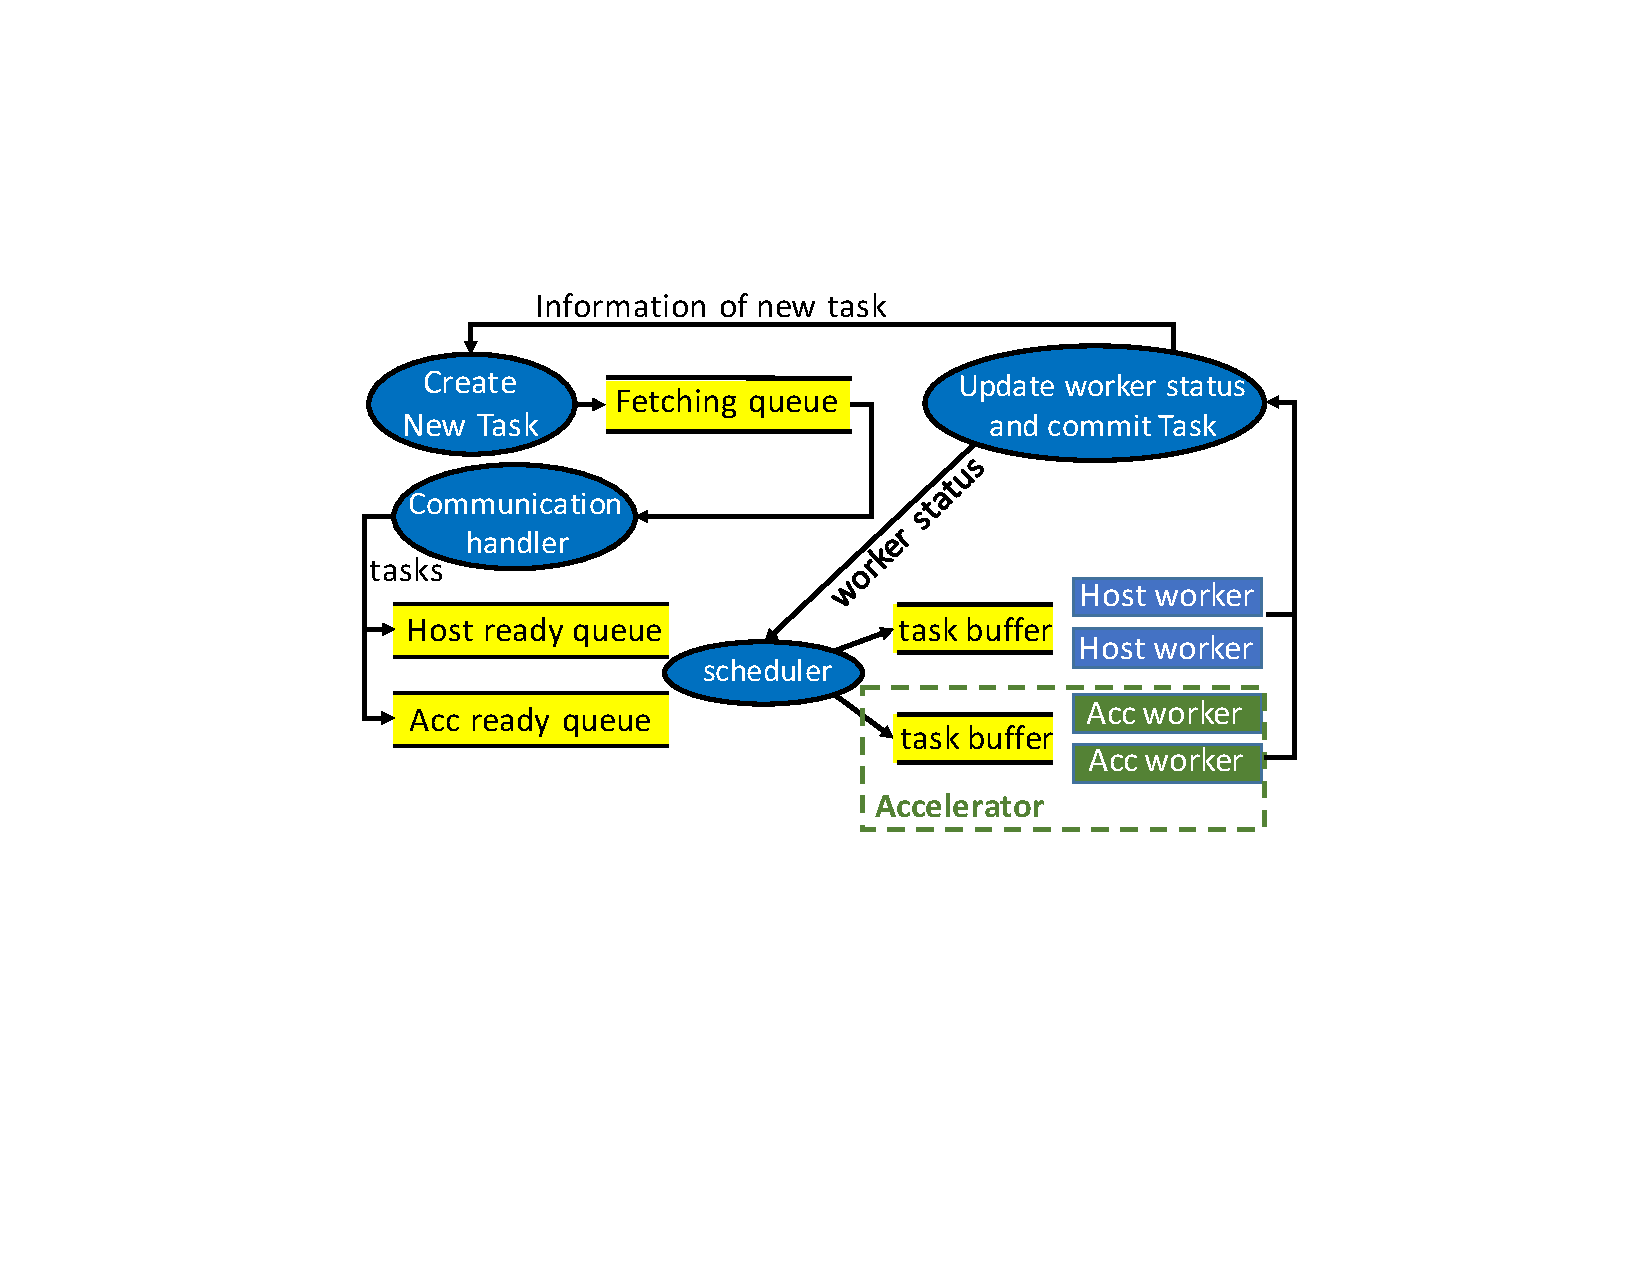
\includegraphics[width=.6\textwidth]{figures/impl.pdf}
\caption{Runtime implementation}
\label{fig:impl}
\end{figure}


\begin{figure*}[htb]
\centering
\subfloat[When direct communication is not available, data are asynchronously fetched through hosts
\label{fig:handler}]{
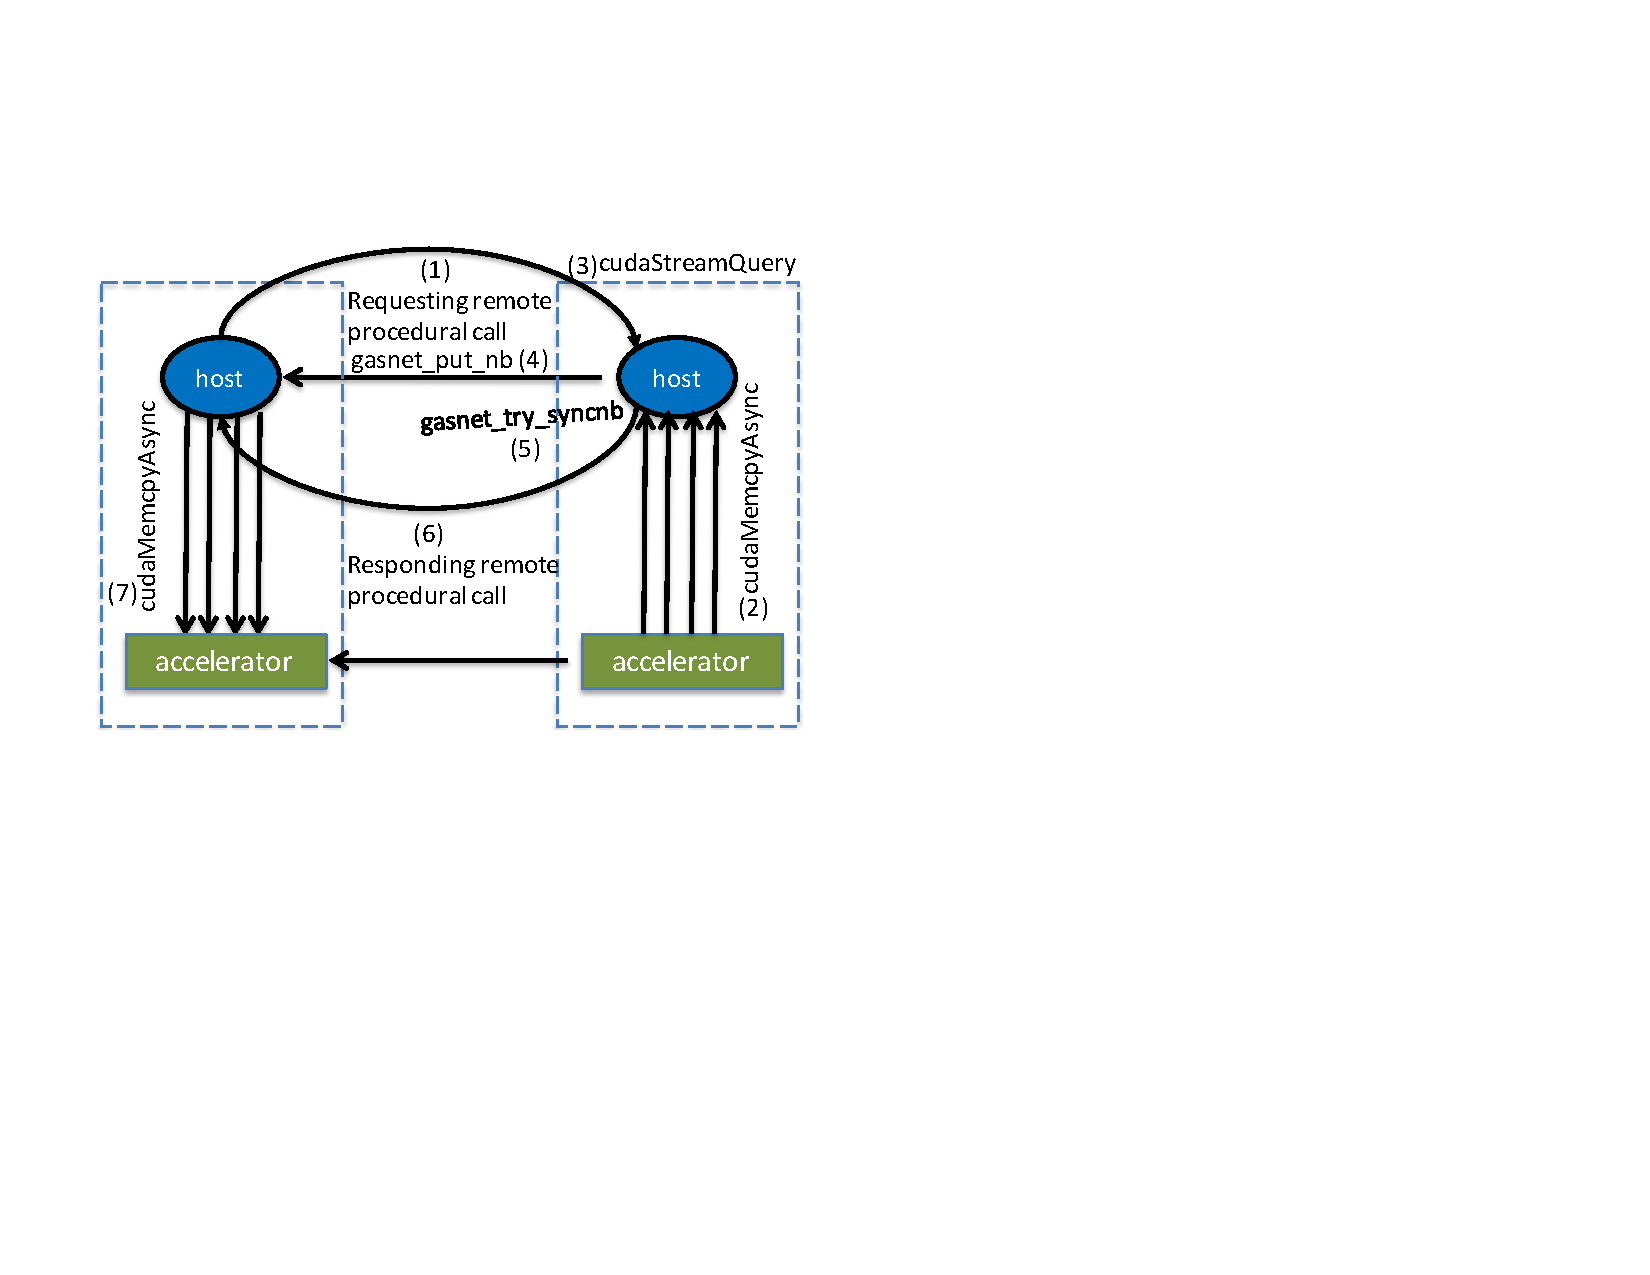
\includegraphics[width=0.42\textwidth]{figures/handler.pdf}
}\hspace{1cm}
\subfloat[The handler supports direct communication if hardware allows
\label{fig:handler_direct}]{
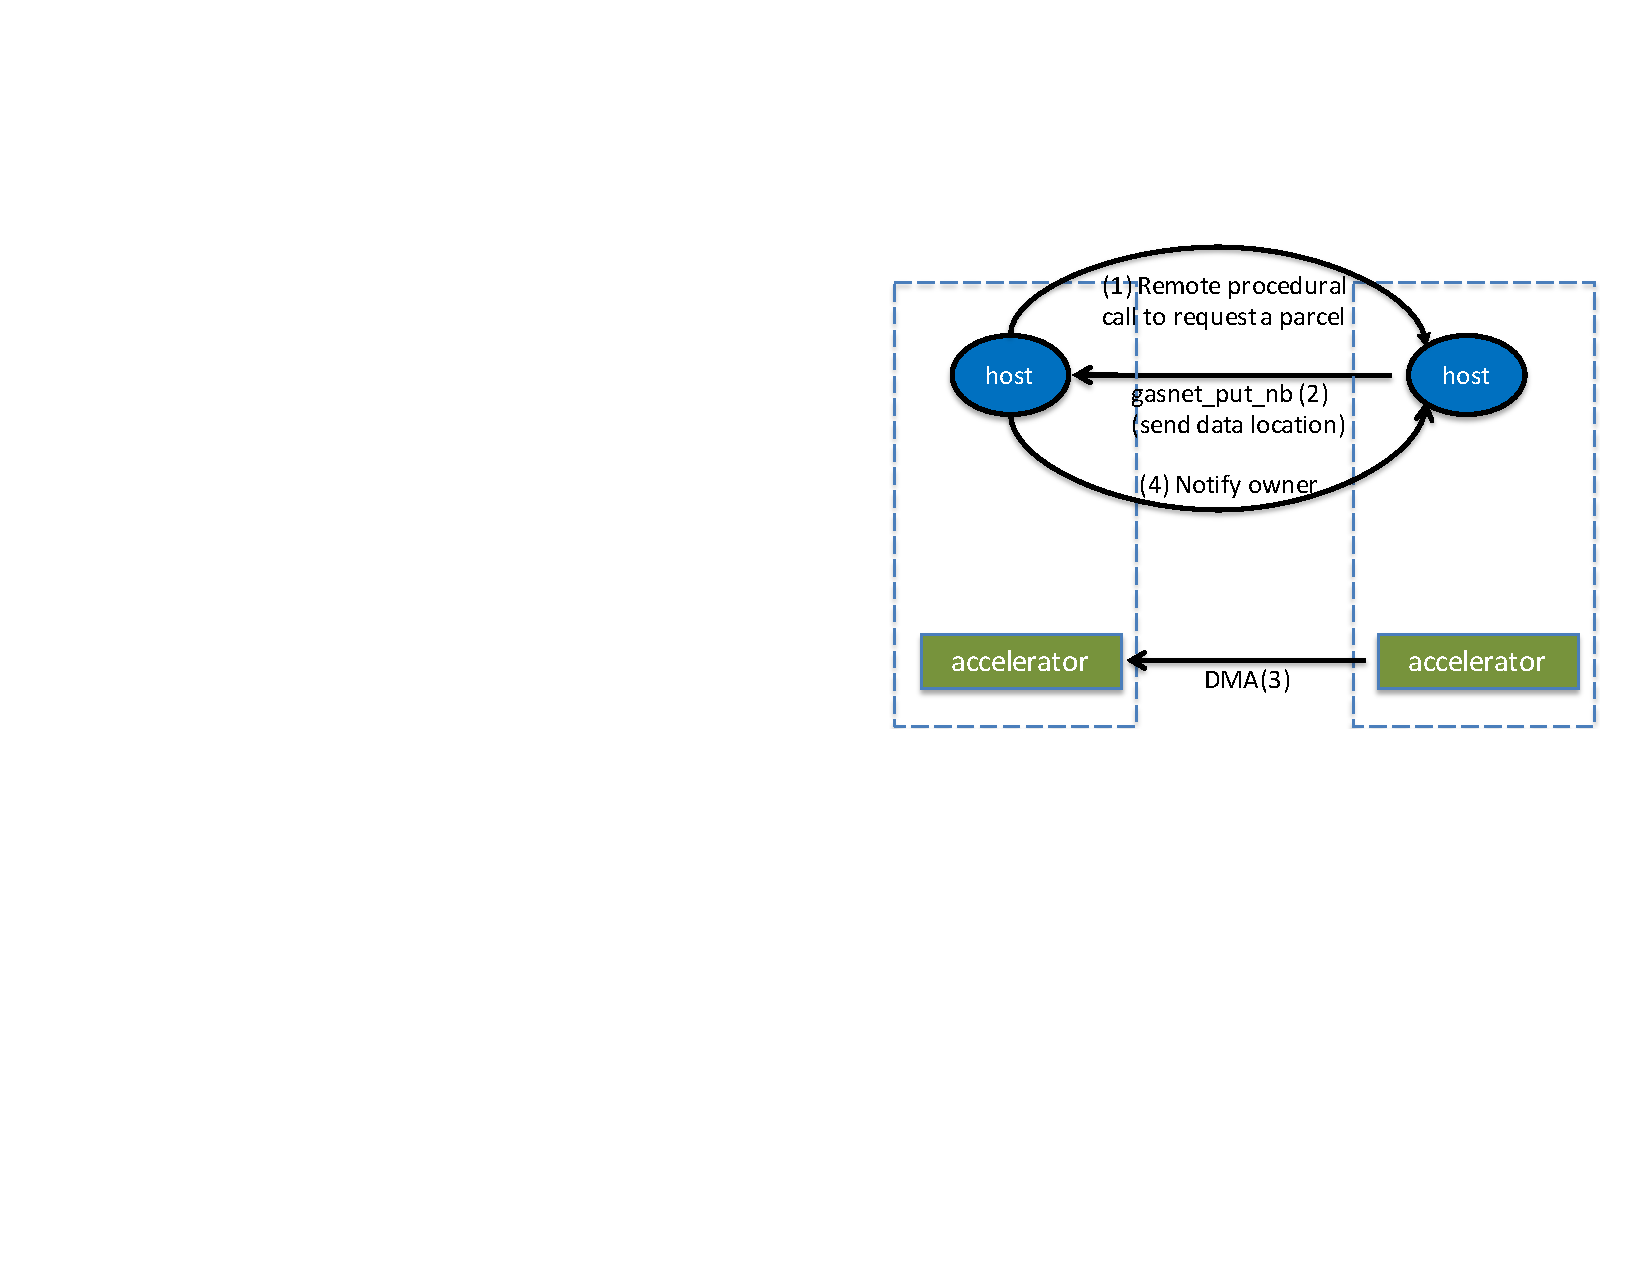
\includegraphics[width=0.42\textwidth]{figures/handler_dma.pdf}
}
\caption{Implementation of the inter-process communication handler}
\end{figure*}

\subsection{Task Management System}
Tasks can be created as soon as input data are produced.
The task management system listens for requests from existing tasks to create new tasks.
%A task may own data.
Upon the completion of a task, the task management system may write data back (if necessary) before destroying the task.
If the original data is located in a different locale, the communication handlers will write the data back asynchronously.
For example, if the task executed on an accelerator while the original data resides in host memory, data will be written back to the host, overlapping with other tasks' computations.

\subsection{Communication handlers}
Once a task has been created, it will be pushed to the {\em fetching queue} by the task management system.
The communication handler periodically pulls tasks from this queue and fetches their input data (parcels).
Depending on the available memory resource, a certain number of tasks in the {\em fetching queue} will be served at a time.
Parcels can be either located in the same process or a remote process.
In the former case, the handler can just pass a pointer if described by the programmer in the task's input.
Otherwise the handler allocates a buffer, packs the data into the buffer and hands it to the task.
In the latter case, parcels can be routed through the hosts or moved directly between accelerators if supported by the hardware.

\subsubsection{Routing parcels through hosts}
%On Intel's KNC-based nodes, we use COI (Coprocessor Offload Infrastructure)\samW{citation for COI??}.

We employ GASNet to implement the inter-process communication.
The process of fetching parcels from a remote process is shown in Fig.~\ref{fig:handler}.
To fetch remote data for a task, the corresponding GASNet process issues an active message (remote procedure call) to request data from the process that owns the data (1).
This procedure looks for the appropriate data at the remote process.
If the data resides in accelerator memory, the procedure also has to pull the data up before sending it (2).
We employ the data transfer primitive provided by the accelerator's vendor to move data to the host.
In particular, on compute nodes with NVIDIA GPUs, we use CUDA stream to move data between host and GPUs.
To avoid blocking the runtime, we do not use any synchronization.
Instead, the communication handler periodically tests the completion of communication activities.
Once the memory transfer from accelerator completes (3), the data can be sent to the requester using a one-sided {\em put} operation (4).
Once the remote GASNet process finishes the remote data transfer, it issues an active message to push the data to the accelerator of the requester (if necessary) and notify the requester when data is available for the task.
All of these activities run asynchronously, and we use a polling mechanism to avoid blocking the runtime.
The reverse process of writing back data produced by the task is similar to the fetching process, and it is also handled asynchronously.



% JohnB: removed since this is unimplemented future work. No sense in cluttering up the pre-results narrative.
\subsubsection{Pulling parcels directly}
When the hardware supports direct communication among accelerators (e.g. via shared PCIe or NVlink), the communication handler can be configured to communicate data on the direct path.
Fig.~\ref{fig:handler_direct} shows that the communication process has been simplified significantly if direct communication is available.
Indeed, the data owner process only needs to respond to parcel requests with the address of the parcel.
Specifically, within a compute node if peer access among accelerators is enabled via a PCIe bus or NVLink connection, GASNet processes exchange information about a shared memory segment at the beginning of the program.
Then they only need to transfer an offset of the parcel, which allows the recipient to pull the data directly.
%In the case of accelerators located on different compute nodes, parcels can still bypass the host memory using RDMAs.
%Specifically, data can be transferred to the NIC without being staged to host memory.
%The RDMA support in RambutanAcc is still under development though (using MPICH as the communication backend).
%In the future, we can also use GASNet as the communication backend when it supports this feature.


\subsection{Task Scheduler}
Tasks become {\em ready} and pushed in the host's {\em ready queue} once all of their data have been fetched.
Each host process runs a task scheduler to dispatch ready tasks to workers. On the GPU, there are
dedicated private task queues per SM and thread block pair. The host's scheduler is responsible
for draining the ready queue into available slots on the finitely-sized worker queues.

%\subsubsection{Task Buffer}
%To keep workers busy, the scheduler frequently checks the runnable task queue and the status of workers.
%However, the task scheduler may not be very responsive since the communication handlers also run on the same processor core.
%Thus, each worker has a private task queue with a few slots.
%The scheduler fills up these slots while the workers keep popping tasks and executing.
%To reduce synchronization overheads, we use a lock-free implementation for this single producer-multiple consumers scheme.

\subsubsection{Accelerator workers using CUDA persistent kernel}
Since the host worker implementation is straightforward, we now present the implementation of accelerator workers on GPUs.
At the beginning, the runtime launches a CUDA kernel to set up workers on the GPUs' SMs and execute assigned tasks.
Once the kernel is launched, CUDA thread blocks find out what SM they are mapped to by the CUDA runtime.
Accessing this information is possible by inserting PTX code to read a special register that holds the SM ID.
%As shown in Fig.~\ref{fig:kernel}, 
We keep only a certain number of thread blocks per SM (this number can be set via an environment variable and the default value is 1).
The reason is that thread blocks run until the program completes and the CUDA runtime co-runs only a limited number of thread blocks on the same SM.
In practice we often use two thread blocks on an SM (if supported) to hide the DRAM latency.
The alive thread blocks will be divided into workers.
Each worker is a group of thread blocks, acting as the new CUDA grid for scheduled tasks.

%\begin{figure}[htb]
%\centering
%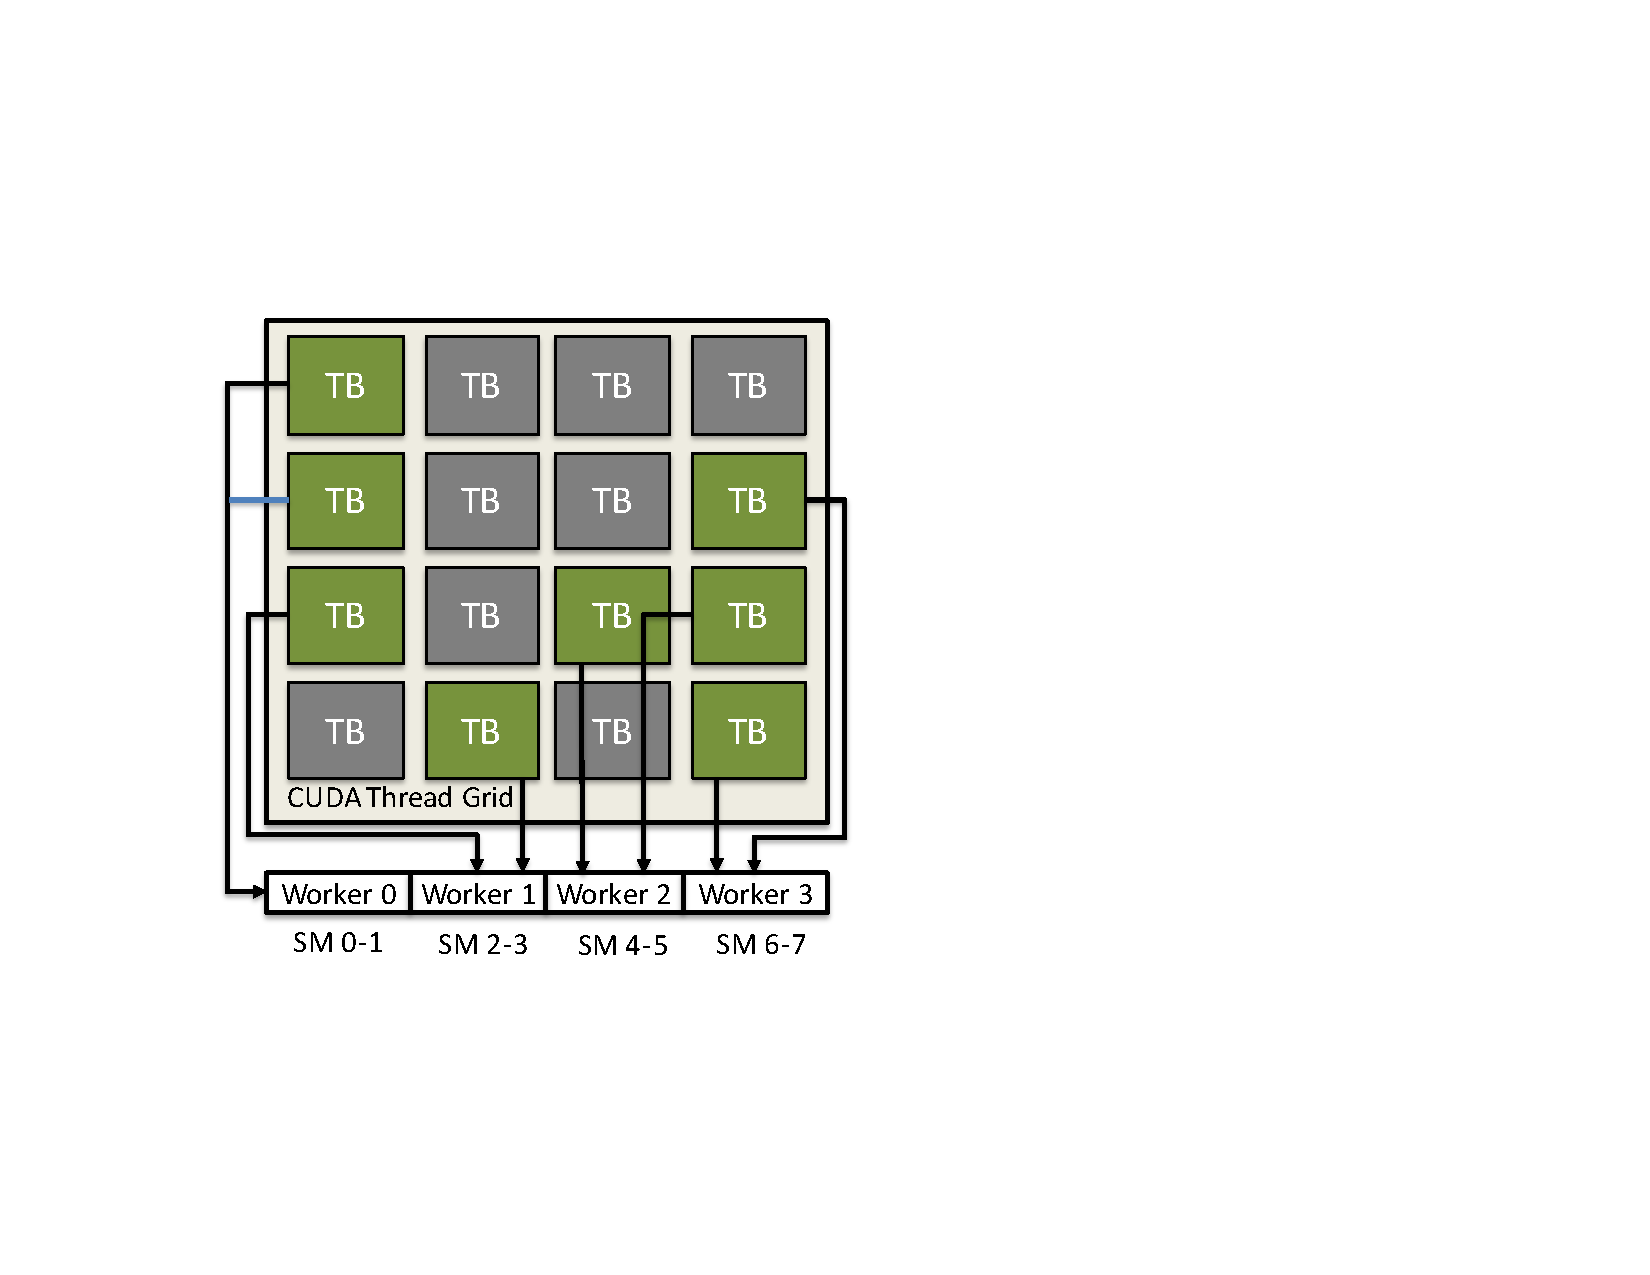
\includegraphics[width=.35\textwidth]{figures/kernel_init.pdf}
%\caption{The persistent kernel selects only a limited number of thread blocks per SM (green color). The default number of thread blocks per SM is 1. 
%In practice, however, we set it to 2 to hide DRAM latency.
%The alive thread blocks are divided into workers to execute tasks.}
%\label{fig:kernel}
%\end{figure}

Now each thread block knows which worker it belongs to and where to find tasks to execute.
Once there are ready tasks and an available worker slot, the scheduler may offload a task (a function and arguments) to task buffers on the GPUs.
Then the scheduler picks a worker and notifies it by writing a signal to the GPU using the non-blocking copy {\em cudaMemcpyCpyAsync}.
If the worker is busy at the time, it will read the signal and execute the corresponding task later.
Once the task finishes, the worker notifies the scheduler.
Since a CUDA kernel cannot explicitly send data to the host, we have to use UVM (unified virtual memory).



\section{Experimental Results}
\label{sec:results}
\subsection{Experimental Testbed}
In this section, we employ the task-based runtime to study the impact of various code optimizations.
We take two benchmarks commonly used in science and engineering: sparse Cholesky factorization and 3D Stencil.
%For sparse Cholesky Factorization, we develop our own CUDA kernels for the sparse matrix multiply update $C = \alpha (A \cdot B) + \beta C$ where $B$ and $C$ are sparse and $A$ is either sparse or dense.
%In these kernels, we perform many optimization techniques such as memory coalescing and spatial tiling.
%We also employ a warp-based thread reduction implementation that minimizes memory accesses.

We use up to three K80 GPUs.
A K80 GPU pairs two GPU devices each having 2496 CUDA cores organized into 13 SMs.
The whole K80-based system is equipped with 24GB DRAM with up to 480 GB/s memory bandwidth.
%For cluster-level optimizations, we run our code on the K20x GPUs on Titan.
%Each K20x is about a half of a K80 in terms of core count and memory bandwidth.
We use the {\tt nvcc} compiler version 7.0 and sm\_35 capability for CUDA codes and the gcc compiler for codes running on the host.
%For experiments on multiple GPUs (on the same node and across nodes), we run experiments on NVIDIA P100 GPUs (the newest generation named Pascal) on SummitDev at Oak Ridge National Laboratory.
%Each Pascal GPU consists of 3584 cores and supports 720 GB/s memory bandwidth.
%A SummitDev compute node consists of four Pascal GPUs.
%These nodes are connected by the InfiniBand interconnect.
%Nvcc 8.0 and sm\_60 are used for experiments on Pascal GPUs.
We use GASNet for communication among the GPUs. 


\subsection{Scheduling tasks on SMs of a GPU}
We first study the significance of optimizations at the GPU level using sparse Cholesky factorization.
For this study we use a GPU of the Kepler K80 card.

\subsubsection{Sparse Cholesky Factorization}
Sparse Cholesky Factorization A= $LL^T$, where A is a sparse and symmetric positive-definite matrix,
appears in many scientific and engineering problems.
Depending on the sparsity pattern of the input matrix, many sparse representations can be used.
In this paper we employ the CSC (Compressed Sparse Column) format. 
The input matrix is organized as a list of "non-zero" tiles, each including lists of non-zero elements and their row and column indices.
The factorization operation is comprised of three smaller kernels: {\em factor}, {\em solve}, and {\em update}.
These computations on CSC tiles and their data dependencies can be represented by a DAG as we previously showed in Fig.~\ref{fig:cholesky}. 
For very sparse matrices, this DAG may consist of many small tasks.
Thus, this is a perfect application to evaluate the benefit of fine-grained task scheduling in increasing the accelerator throughput.
We place data on the host's DRAM and execute {\em factor} and {\em solve} on the host's worker.
The compute-intensive {\em update} kernel is executed on the GPU workers.
The runtime automatically streams data required by this kernel to the GPU's DRAM and streams the results back.

%An interesting path to explore is the tradeoff between coarse and fine-grained scheduling policies.  
%For sparse Cholesky, the matrix is represented by many small CSC tiles.\samW{the previous sentence repeats the one}
%Thus, even a small problem size can result in many tasks.
We implemented two code variants, which differ from each other in the method of task execution used (refer to Section~\ref{sec:task-def} for {\em task type} descriptions).
The first code variant implements the {\em Update} phase with {\em type-3} task to launch the sparse matrix multiply kernel on the whole GPU, and hence the name {\em CUDA Launch}.
The other code variant is called {\em persistent kernel}, since it employs {\em type-2} task, which can be scheduled on a group of SMs by the persistent kernel.
Fig.~\ref{fig:coarseFine} shows results of sparse Cholesky under two scheduling policies.
It can be seen that {\em persistent kernel} outperforms the coarse-grained {\em CUDA Launch} policy.
This can be explained as follows.
Each CSC tile is very small (e.g. 32$\times$32), making it hard to map computations efficiently to many CUDA cores.
Thus, it may not be possible to scale a task to all available SMs of a GPU.
We observe that for many input matrices tasks run more efficiently after reducing the number of SMs per worker by a factor of 2$\times$ or 4$\times$.
Since there are many tasks that can be runnable at a time, the scheduler can keep all SMs busy at very small overhead.
Fig~\ref{fig:nWorkers} shows the optimal number of workers on a K80 GPU for sparse Cholesky Factorization when the degree of sparsity of the input matrix varies.
If the sparse matrix is filled with many tasks we have more parallelism, allowing us to configure the GPUs with more workers.
Note that we picked these three numbers to represent wide ranges of sparsity, and the actual number in practice may fall somewhere in these ranges. 


\begin{figure}[htb]
\centering
\subfloat[Since tile size is small (32$\times$32), co-scheduling tasks on the same GPU with the persistent kernel improves performance
\label{choleskySche}
]{
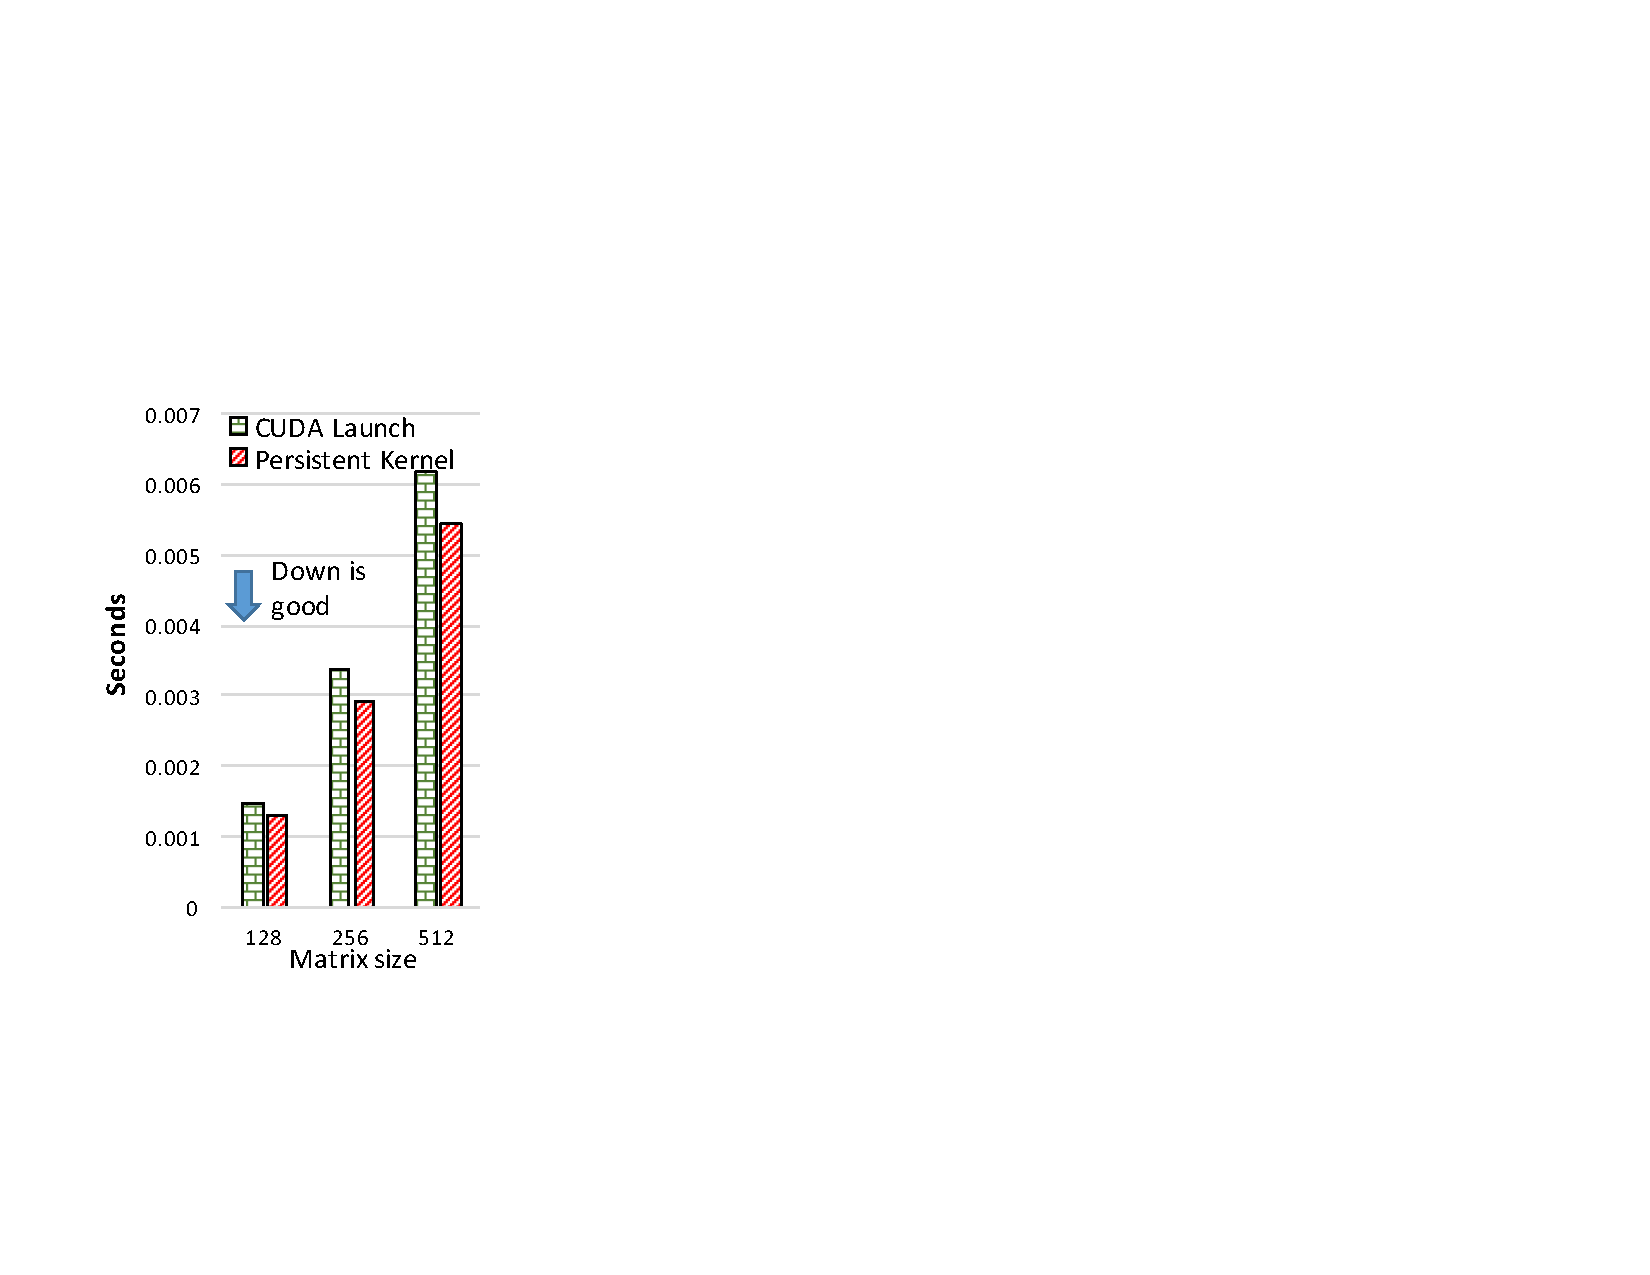
\includegraphics[width=0.35\textwidth]{figures/choleskyScheResults.pdf}
} \hspace{1cm}
\subfloat[If there is enough parallelism (matrix is filled with more non-zeros), increasing \#workers may increase performance
\label{fig:nWorkers}
]{
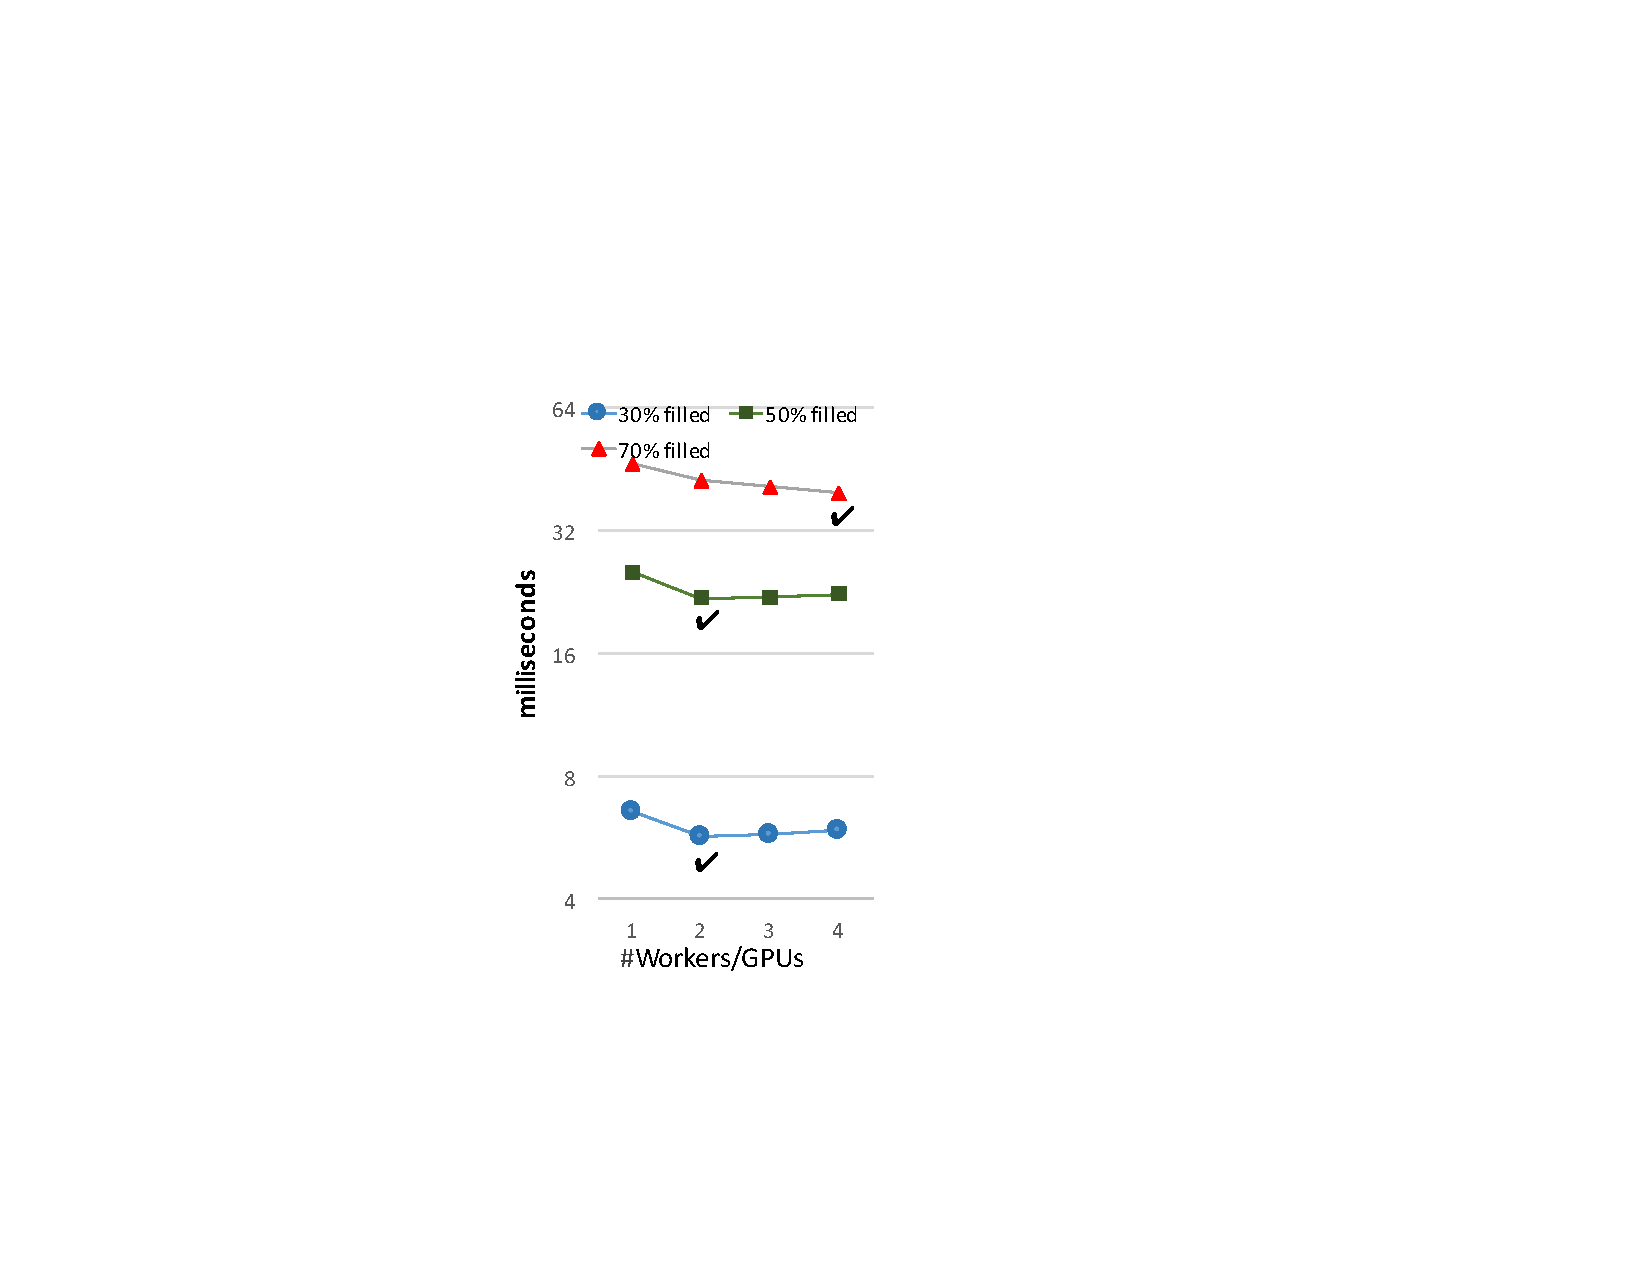
\includegraphics[width=0.35\textwidth]{figures/nWorkers.pdf}
}
\caption{Sparse Cholesky Factorization: Left: the persistent kernel with two workers/GPU improves the performance. For this experiment, the degrees of sparsity are low (under 30\%). Right: for matrices with higher degrees of sparsity, increasing the number of workers  may further improve the performance}
%\samW{note left vs. right;  for left, what is the sparsity???  where does the matrix come from???}}
\label{fig:coarseFine}
\end{figure}

The lesson learned from this study is that fine-grained scheduling can be very helpful if we have a DAG with many small tasks, which cannot effectively utilize the whole GPU.
The persistent kernel also allows running multiple task types simultaneously, taking advantage of additional task parallelism compared to sequentially launching uniform accelerator kernels, all at a small programming cost.
Using these methods, the programmer can obtain high compute throughput on GPUs without complicating the application algorithm, which is an important capability since sparse representations are very common in practice.

%\subsubsection{Viola-Jones Face Recognition}
%\samW{is there a citation for this code/algorithm}
%We next study the impact of dynamic task scheduling in balancing the workload among SMs of a GPU.
%For this study we use the Viola-Jones face detection kernel~\cite{facedetection1, facedetection2}, an important module in many applications such as security surveillance.
%The Viola-Jones face detection algorithm detects faces by scanning a rectangular window of pixels over the image where it looks for features of a human face. 
%If a window contains a significant number of these features, it is accepted (considered to contain a face).
%Since face size varies, the window is scaled a number of times and the scanning process is repeated. 
%To reduce the number of features that each window needs to check, the window passes through a number of different stages. 
%Early stages have fewer features to check and are easier to pass, whereas later stages have more features and are more selective. 
%At each stage, if the window's features do not exceed a threshold, the window is immediately rejected, skipping further stage processing.


%\begin{figure}[htb]
%\centering
%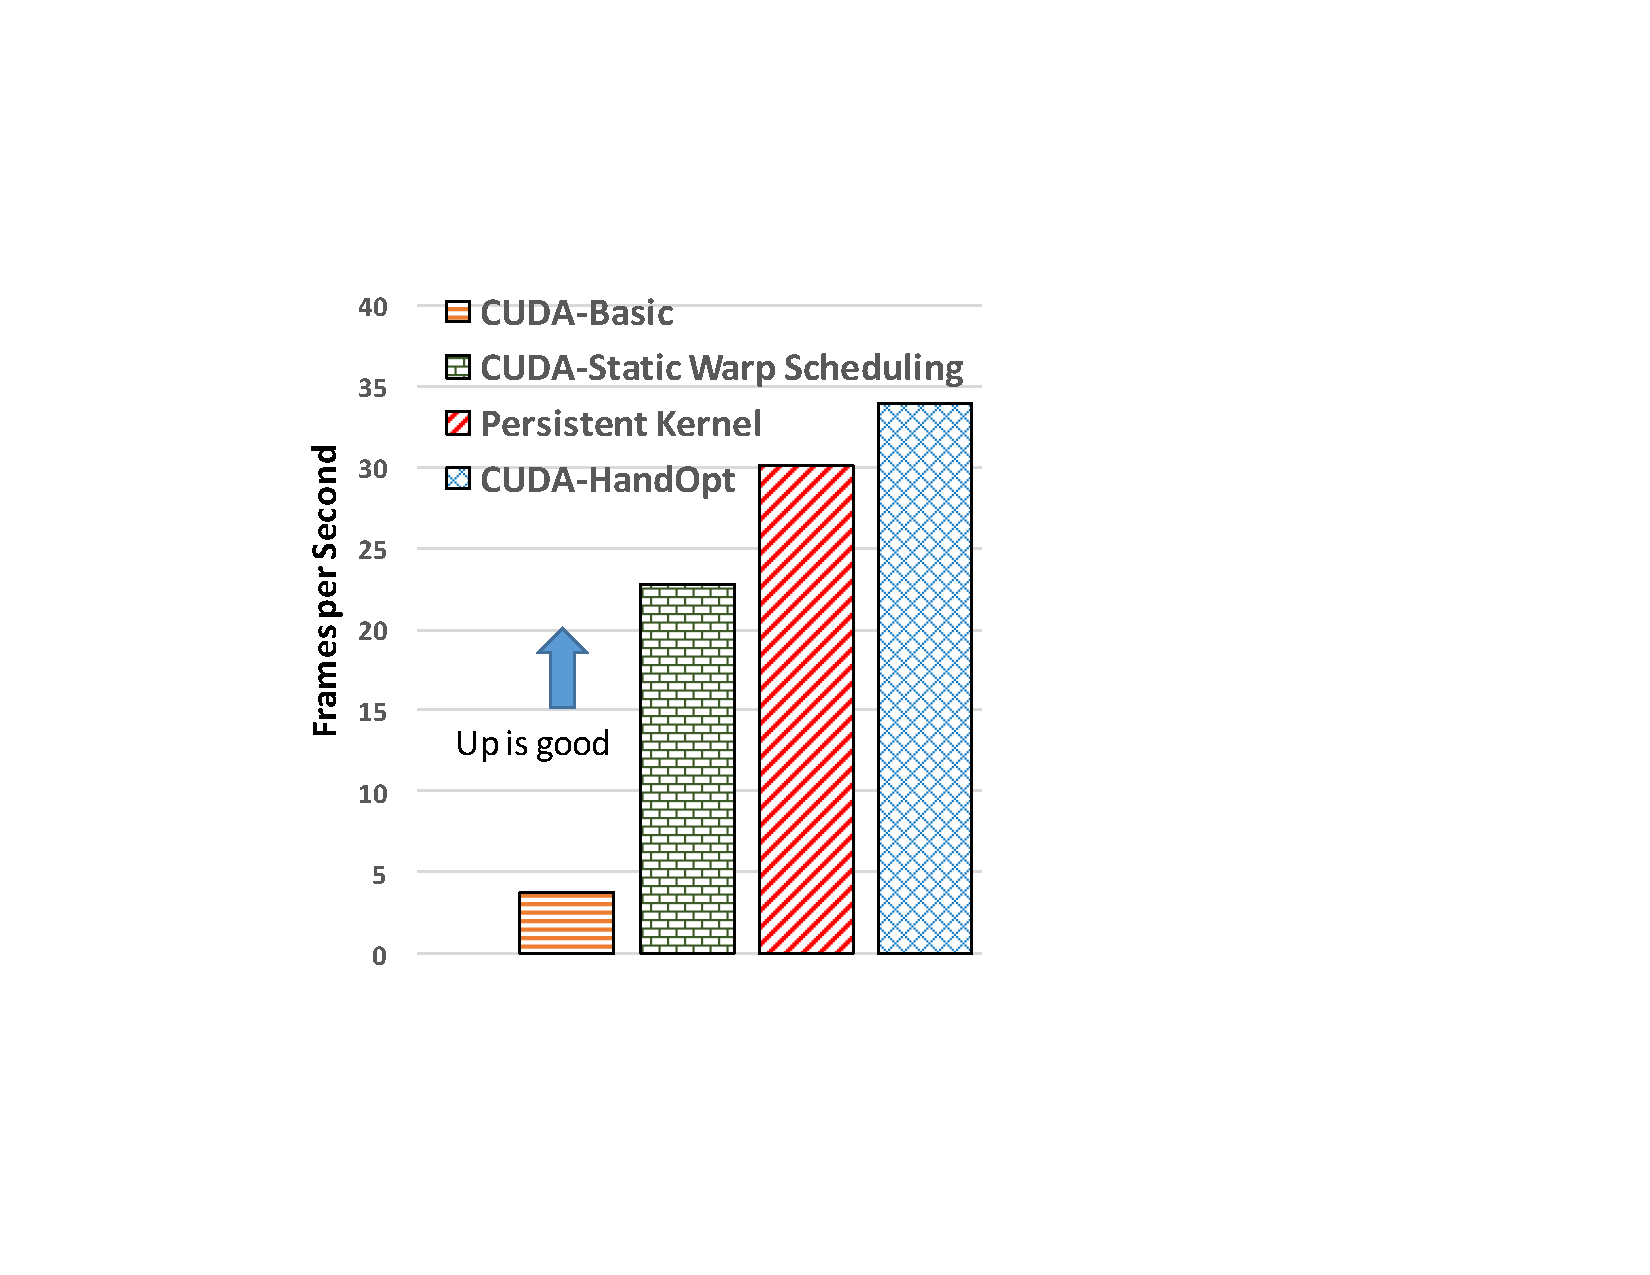
\includegraphics[width=0.35\textwidth]{figures/faceRecognition.pdf}
%\caption{Viola-Jones Face Recognition: Although the warp scheduling implemetation boosts up performance of the face detection algorithm via eliminating thread divergence, there remains substantial load imbalance among warps. The persistent kernels allows tasks to be dynamically scheduled to workers. Within each worker, task's workload is further split dynamically to warps. The performance of the persistent kernel is very close to that of the hand optimized code}
%%Balance the face searching\samW{what is FPS?  I assume up is good... i.e. FPS is a throughput rather than time metric}}
%\label{faceRecognition}
%\end{figure}




%\begin{figure*}[htb]
%\centering
%%\begin{subfigure}[b]{0.45\textwidth}
%\subfloat[A and B dependencies on each replication layer
%\label{deps}]{
%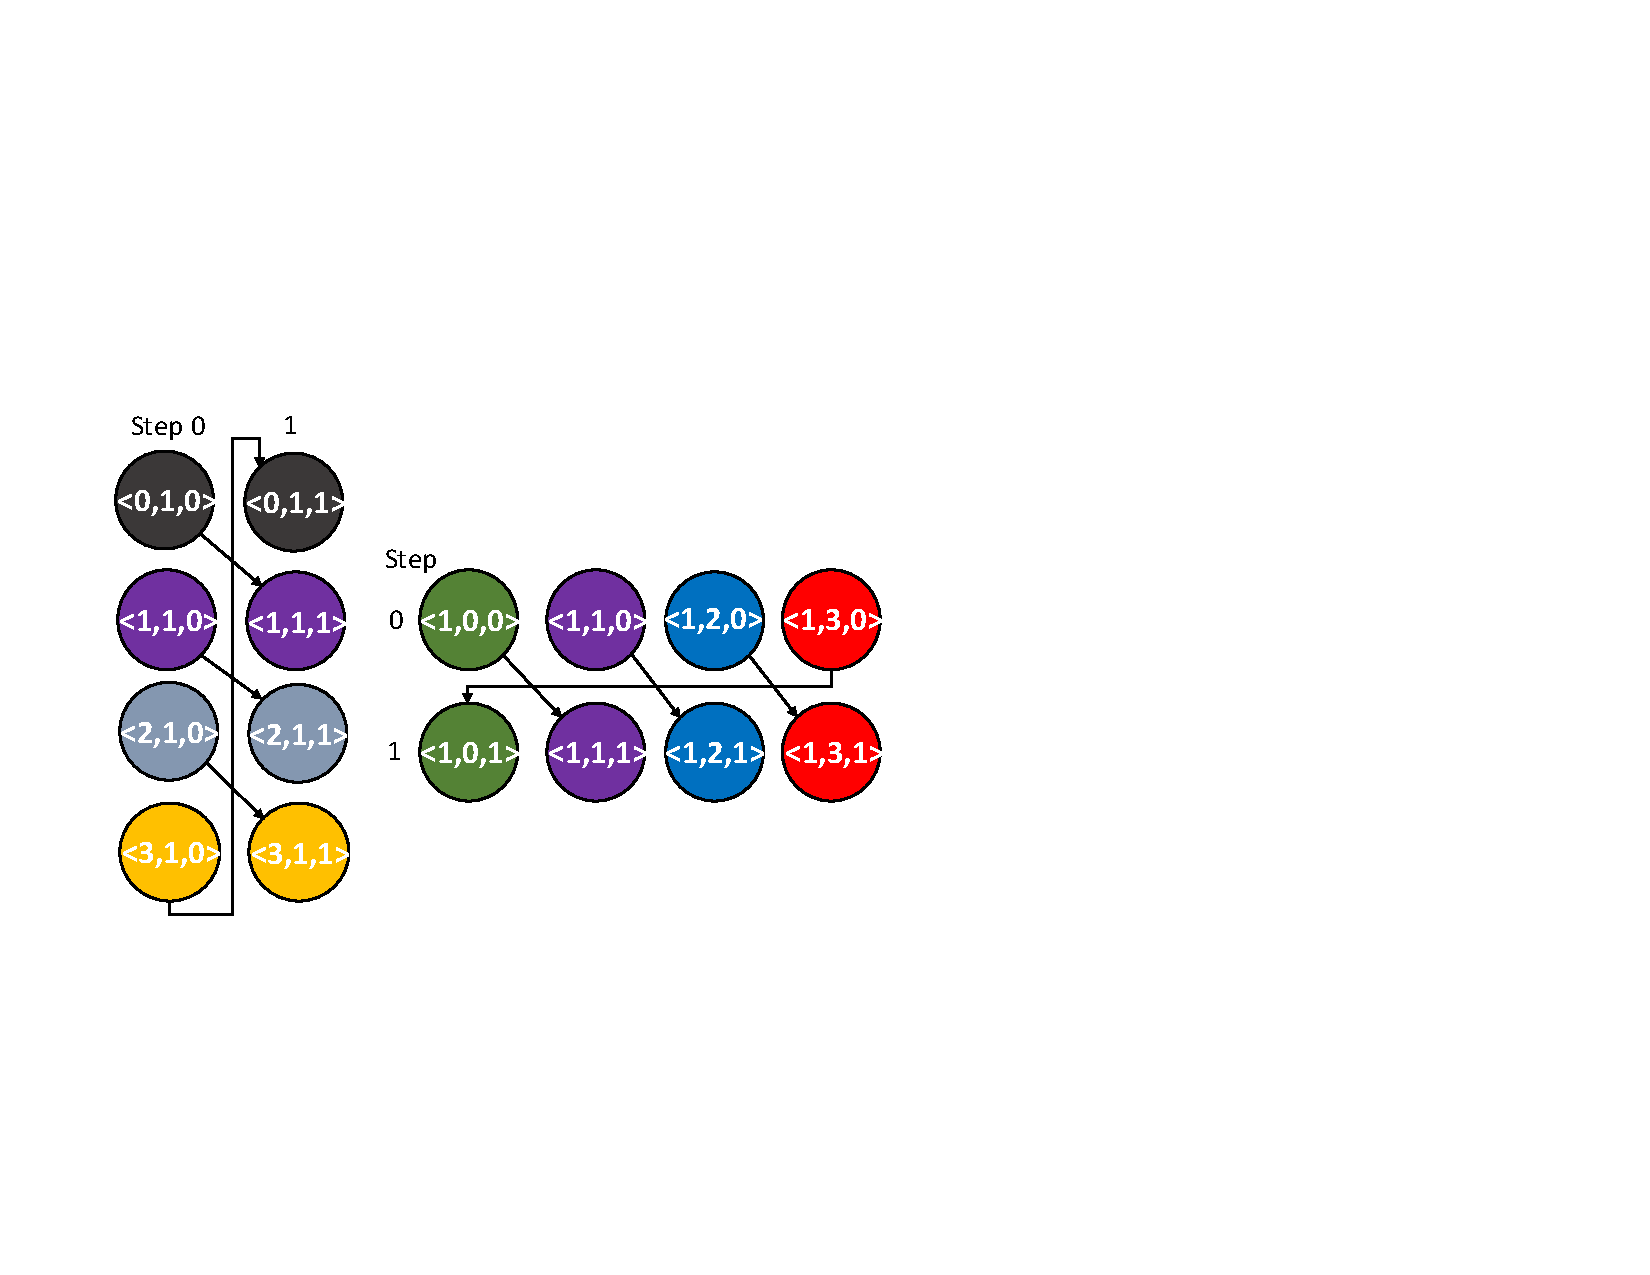
\includegraphics[width=0.45\textwidth]{figures/cannon0.pdf}
%}
%%\begin{subfigure}[b]{0.37\textwidth}
%\subfloat[Results are reduced to the original layer
%\label{dataspace}]{
%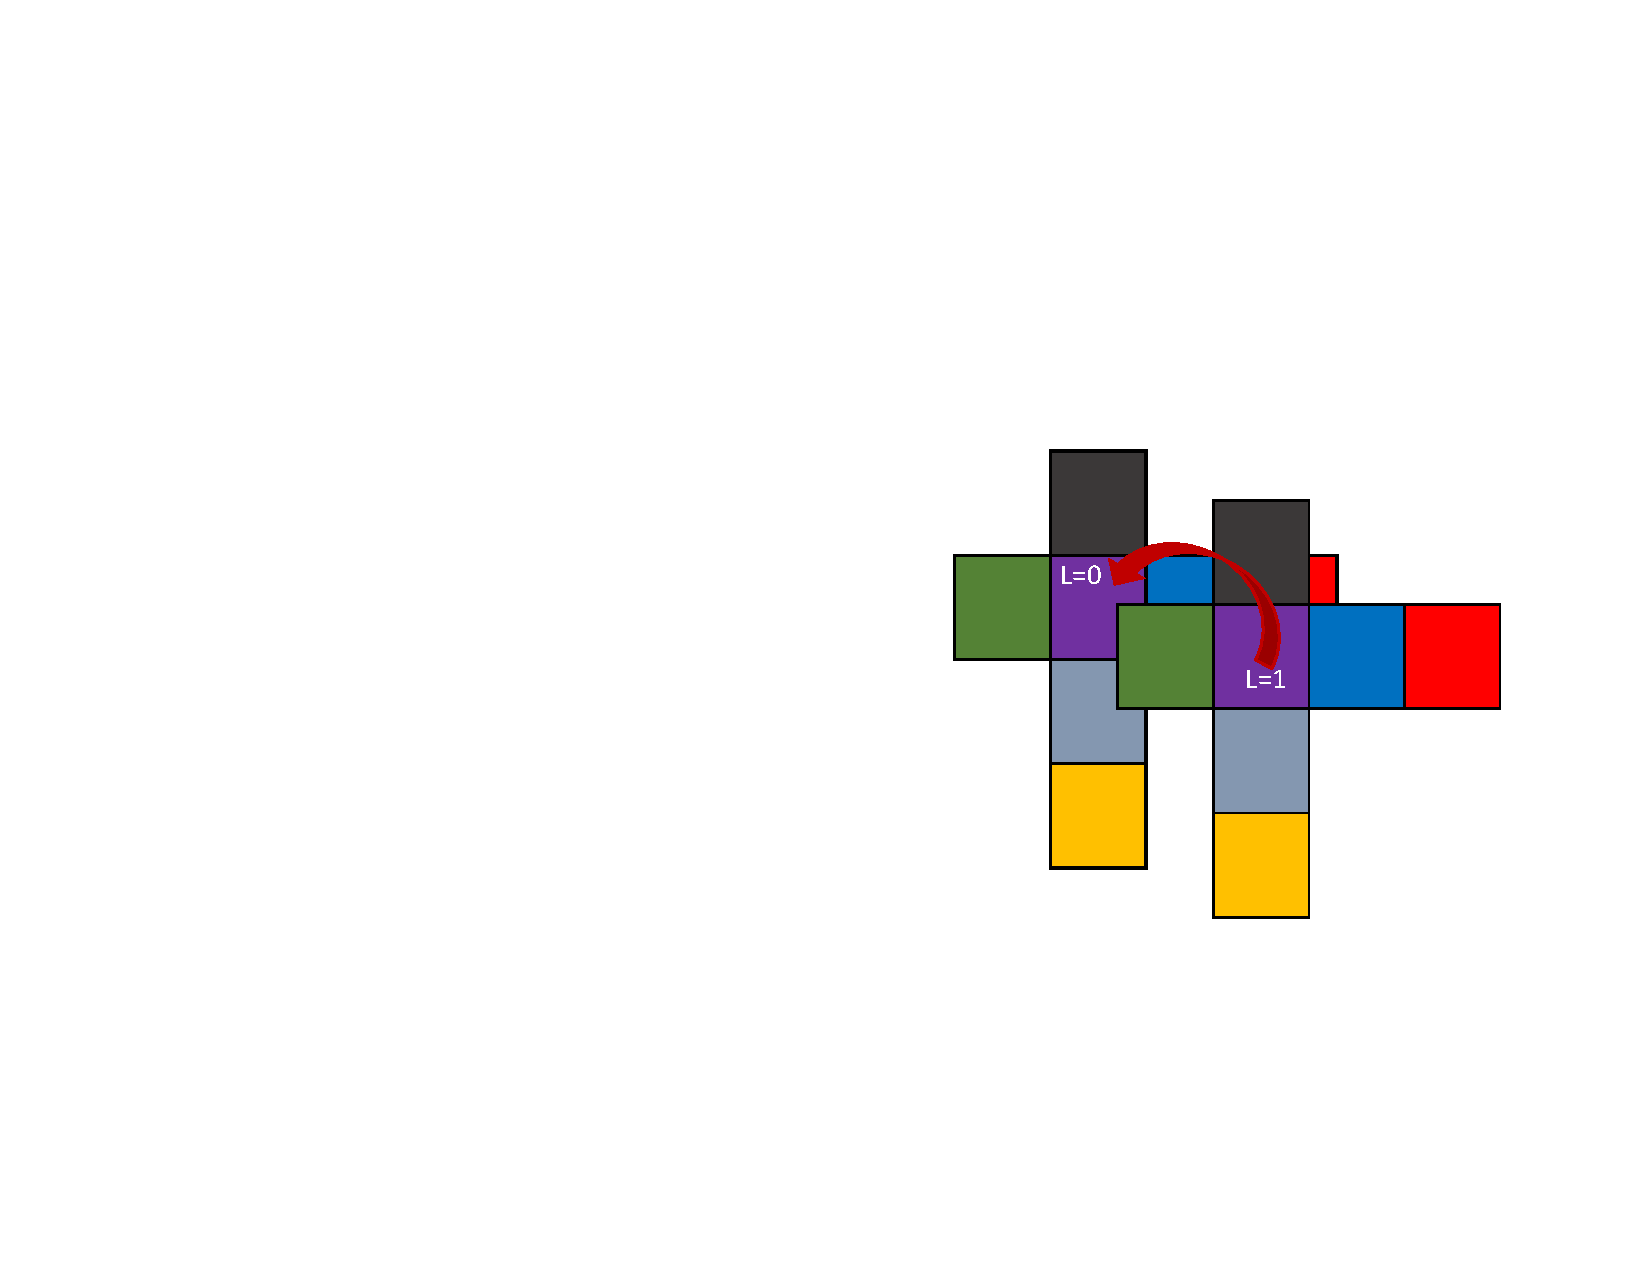
\includegraphics[width=0.37\textwidth]{figures/cannon1.pdf}
%}
%\caption{Computing $C= \alpha A * B + \beta C$ using the 2.5D Cannon's matrix multiplication algorithm given the input matrices are already replicated and aligned. 
%The DAG partitions matrix C and the step space of the algorithm.
%Task Id is a triple where the first two numbers represent the coordinates of a C partition and the last is the step number of the algorithm. 
%Fig.~\ref{deps} shows two subsets of the graph to illustrate two types of data dependecies required to compute C.}
%\label{fig:25DCannon}
%\end{figure*}


%We use a few code variants presented in \cite{facedetection_dws}.
%For this application, it is straightforward to exploit parallelism among search windows.
%Each CUDA thread block is responsible for a fixed number of windows, which will be further distributed to threads within the thread block.
%In this paper we call this code variant {\em CUDA-Basic}.
%Since the number of instructions per window depends on the input, the impact of thread divergence is expected to be significant.
%Thus, we also employ a {\em CUDA-Static Warp Scheduling} version which allows 32 threads in a warp to share a window (and thus they perform the same number of instructions).
%We then port this code on our runtime using {\em type-2} tasks, hence we call it {\em persistent kernel}.
%We expect to improve the performance further by balancing the workload among these warps.
%Finally, we run a hand-optimized code variant previously developed in \cite{facedetection_dws}.
%This variant effectively embeds the task scheduler into the kernel code and has capabilities similar to our runtime's scheduler,
%but at lower cost since the task scheduler is specialized and runs on the GPU.

%Fig.~\ref{faceRecognition} shows the performance of all code variants.
%{\em CUDA-Basic} performs poorly as expected.
%Under this na{\"i}ve strategy, a few threads progress through more feature detection stages while most threads reject their window early and start with a new window, causing thread divergence.
%%since there is no chance to detect a face in their current windows.
%Since the CUDA runtime runs the 32 threads of a warp in lock-step, the diverged threads must be serialized.
%%\samW{previous sentence is unclrear...  Are you saying the naive code has a thread divergence problem?}
%This explains why {\em CUDA-Static Warp Scheduling} improves the performance significantly.
%However, there remains significant load imbalance among warps.

%With {\em persistent kernel}, windows are distributed to workers dynamically.
%Specifically, we configure the runtime with 26 workers, with one thread block per worker and two workers per SM.
%The scheduler running on the host keeps assigning blocks of windows to these workers.
%In order to hide the scheduling latency, we configure the task buffer of each worker with multiple slots.
%While each worker is processing its current window, the scheduler can offload other windows to the remaining slots.
%In this experiment, each block takes about 50$\mu$s to finish, whereas the offloading cost is around 10$\mu$s.
%Thus, configuring the task buffer with two slots is sufficient.
%Fig.~\ref{faceRecognition} shows that {\em persistent kernel} outperforms {\em CUDA-Static Warp Scheduling} by 1.35$\times$.
%All the performance improvement can be attributed to the capability of balancing computations among SMs of the GPU.
%The {\em persistent kernel} version achieves 90 percent of the hand-optimized version at substantially less programming complexity.
%%\cyC{replace X percent above with the actual number}
%% The {\em CUDA-Hand Optimized} version runs even faster.
%The additional performance of the hand-tuned version is due to reduced overhead from embedding the scheduling logic directly into the application source code.
%%\samW{where did the CUDA versions of the code come from?  Did you write them all?  if not, cite source}
%
\subsection{Scheduling tasks on multiple GPUs}
\subsubsection{3D Stencil}
\label{subsec:3DStencil_1node}
%\samW{3D stencil is an ill-defined term... is this a 7-point, constant coefficient laplacian?  Are you doing a smoother with a RHS?  are you assuming periodic BCs?  or constant(node/vertex centerd) boundaries?}
On multiple GPUs we pick {\em 3D Stencil}, an iterative solver for Laplace's equation in three dimensions.
{\em 3D Stencil} iterates over a 3D mesh, updating data elements using values from six nearest neighbors.
3D stencil is a memory bandwidth bound application. 
Thus, using GPUs can boost up the performance significantly.
%The DAG for this application is similar to that shown in Fig.~\ref{fig:taskGraph}, except for the number of dimensions.
%In particular, each task is associated with a data partition with up to six ghost regions.
%A task can be run when the previous iteration on this data partition finishes and it pulls all the needed ghost regions from neighboring tasks.


%\begin{figure}[htb]
%\centering
%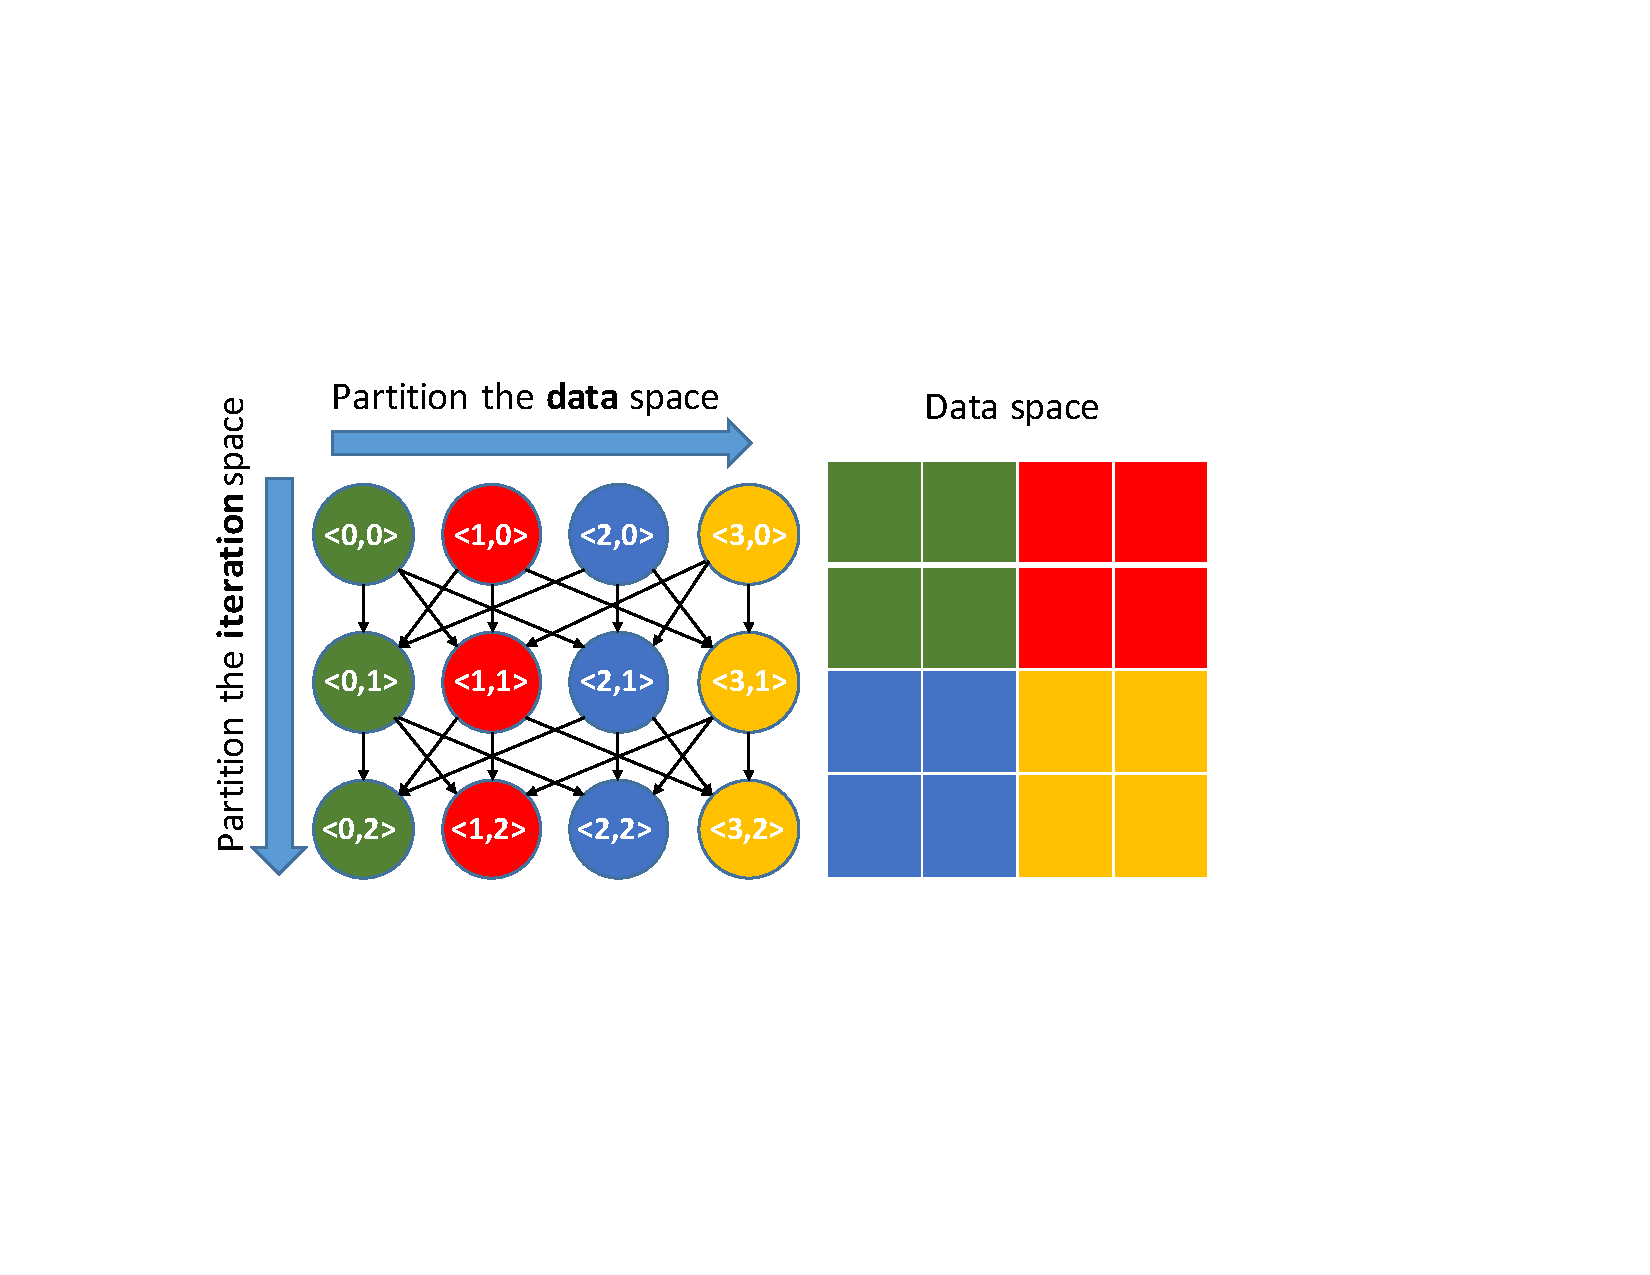
\includegraphics[width=.47\textwidth]{figures/taskGraph.pdf}
%\caption{A directed acyclic graph for a 2D stencil code (which shows the concepts of a 3D Stencil task graph). The graph partitions the data space and the iteration space. Data space is divided into parcels, and the color represents the ownership mapping function (tasks to data parcels).}
%Tasks are fireable as soon as data dependencies are satisfied.}
%\label{fig:taskGraph}
%\end{figure}




\begin{figure}[htb]
\centering
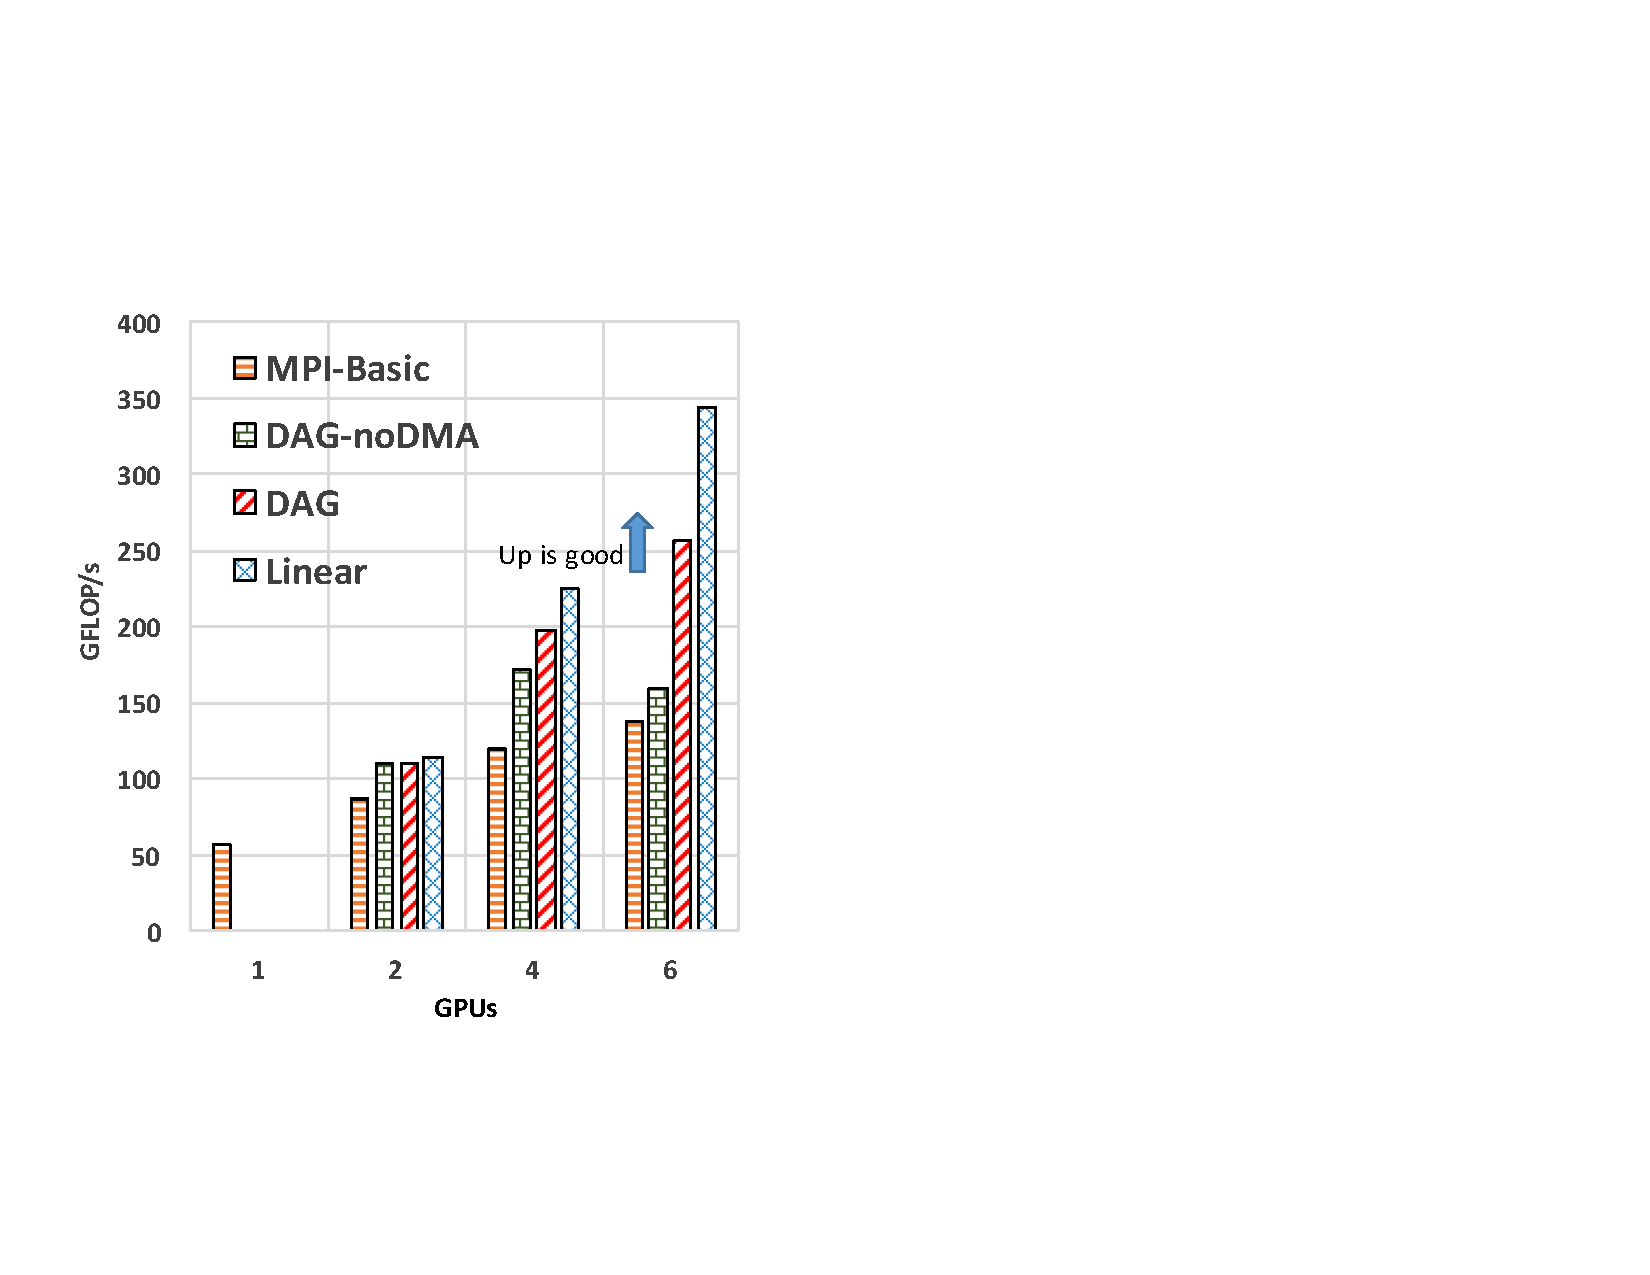
\includegraphics[width=0.7\textwidth]{figures/stencil_single_node_tida.pdf}
\caption{Strong scaling study of 3D stencil on a single compute node with six Kepler GPUs (3 K80 cards) connected via a shared PCIe bus. Problem size $512^3$.}
\label{fig:stencil_single_nodes}
\end{figure}

A challenge for this code is that the communication cost is relatively significant.
Not only does the GPU implementation introduce extra cost of transferring data among host and the GPUs, it also puts more pressure on the communication by improving the computation rate due to its high memory bandwidth.
Thus, it is interesting to use the task-based runtime to study the impact of hiding/lowering such communication costs.
For this study, we implemented four code variants.
The first variant, {\em MPI-Basic} uses blocking CUDA transfers to communicate between the host and GPU, and it uses MPI for communication among hosts.
We port this code to our runtime using {\em type-3} tasks, which offload the same CUDA kernel in {\em MPI-Basic} to the whole GPU.
However, it performs a non-blocking kernel launch with a CUDA stream given by the runtime, allowing the scheduler to manage ready tasks while servicing communication for other tasks.
Using the same task graph, we configure the communication handler of the runtime system with and without direct communication among the GPUs, and hence the names {\em DAG} and {\em DAG-noDMA}, respectively.
The {\em Linear} code variant shuts off all communication in {\em MPI-Basic}, and thus does not produce a correct result.
This variant illustrates the hypothetical performance if {\em all} communication costs were hidden.

Fig.~\ref{fig:stencil_single_nodes} shows the strong scaling performance of four code variants.
We can easily see that the communication has a notable impact on the scalability of {\em MPI-Basic}.
Under this circumstance, hiding communication is always effective whether or not we route data through the host.
{\em DAG} and {\em DAG-noDMA} run at the same rate on two GPUs.
However, on six GPUs we no longer have enough computation to hide the communication cost of the indirect copy.
This explains why {\em DAG} substantially outperforms {\em DAG-noDMA}.
%\samW{Be careful on the previous 2 paragraphs.  There may not be enough NVLink bricks to connect 4 GPUs to a POWER8}




%\begin{figure}[htb]
%\centering
%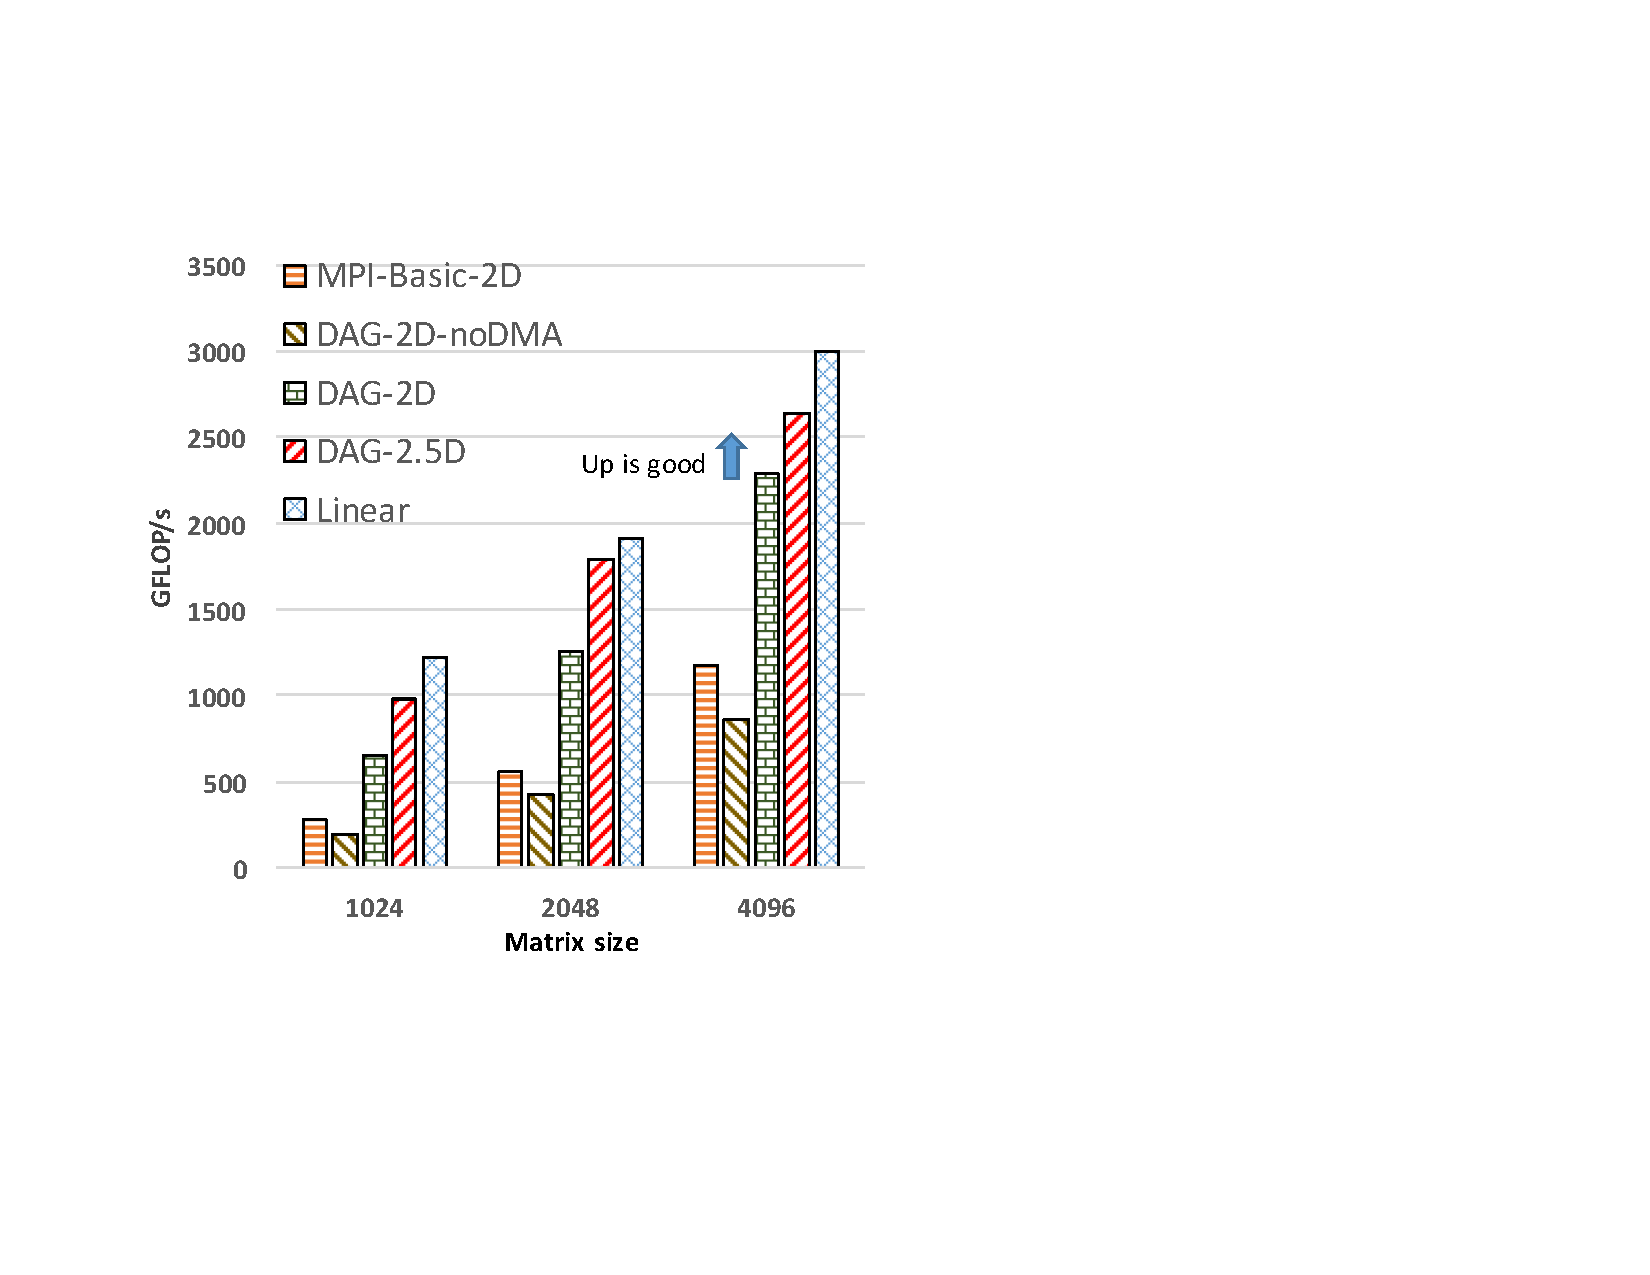
\includegraphics[width=0.49\textwidth]{figures/cannon_tida.pdf}
%\caption{2.5D Cannon on two K80s (four GPU devices)}
%\label{cannon_onnode}
%\end{figure}



%\subsubsection{2.5D Cannon Matrix Multiply}
%Although sparse representations are widely used in practice, dense matrix operations also have a significant share in many scientific and engineering areas.
%As a result, we employ a dense matrix multiplication operation $C = \alpha (A \cdot B) + \beta C$ to evaluate our runtime.
%This is a compute bound kernel, and the GPU architecture is very well suited for the computation. 
%There are many algorithms for the matrix multiply operation, and we use a well-known extension of the standard 2D Cannon's algorithm called {\em Communication Avoiding} or 2.5D Cannon~\cite{25Dcannon}. 
%Under the original 2D Cannon's algorithm, the available tasks are organized into a {\em T=PxP} mesh, partitioning each of the three matrices A, B, and C into blocks.
%These partitions are first aligned using a skewing operation.
%The algorithm then performs P computation steps accumulating the C partition using the rotated A and B partitions.
%The communication avoiding algorithm replicates the input matrices by a factor of L using an additional task dimension.
%The algorithm broadcasts input data to layers in this dimension to compute the traditional Cannon with T/$\sqrt(L^3)$ steps then reduces the results back to the first layer.

%On a single node, we do not have enough GPUs to replicate the mesh of an MPI program.
%Thus, we use a 2D variant of the Cannon algorithm {\em MPI-Basic-2D}.
%To have fair comparisons, we also run the {\em DAG} variant in 2D form where there is no advantage of avoiding communication.
%This variant includes {\em DAG-2D-noDMA} and {\em DAG-2D}.
%To study the total impact of three optimizations (communication overlap, avoiding, and direct communication) we employ {\em DAG-2.5D}.

%Figure~\ref{cannon_onnode} shows the performance of these variants as the matrix size varies.
%It can be seen that the communication overhead is very high in this experiment.
%Generally, matrix multiply operations have high compute intensity;
%however, on GPUs these operations can be processed more quickly than the communication.
%Since communication dominates, the overlapping technique in {\em DAG-2D-noDMA} is not effective.
%The performance is even worse due to the overhead of over-decomposing the problem.
%However, things completely change with direct communication among the GPUs, which
%reduces communication to a level where overlap becomes effective again.
%We can see that the performance is boosted significantly with {\em DAG-2D}.
%{\em DAG-2.5D} is the most interesting case because in addition to the benefit of communication-avoidance,
%% This is not really the original communication avoiding technique because
%we also use ``virtualized'' GPUs (via tasks and workers) to replicate the matrix.
%Thus, we actually realize the benefits from both techniques simultaneously.
%The performance of this code variant is very close to the {\em Linear} performance where all communication is shut off.


%\subsection{Scheduling tasks at the cluster level}
%In Sec.~\ref{subsec:3DStencil_1node}, communication optimization techniques (i.e. communication overlap and GPU direct access) realize modest performance improvement when the NVLink connection is available.
%We now extend the experiment in Fig.~\ref{stencil_single_node_summit} to multiple compute nodes on SummitDev.
%As previously described, a SummitDev node consists of four Pascal GPUs.
%These nodes are connected via an InfiniBand interconnect.
%We reuse 3 code variants in the previous study: {\em MPI-Basic}, {\em DAG}, and {\em Linear}. 
%In this study, we expect the communication to be increased  due to the off-node communication.
%Thus, we also develop a hand optimized code variant called {\em MPI-HandOpt}.
%Like {\em DAG}, this code also over-decomposes the data space into smaller partitions (which called {\em parcel} in {\em DAG}).
%Unlike {\em DAG}, this code statically schedules the CUDA kernel launch and the communication on ghost cells.
%Specifically, after launching a non-blocking kernel to update data elements in a partition (let's say A), the code handles communication for another partition B.
%When the CUDA kernel and data communication both complete, the code launches kernel on partition B and services communication for partition A.
%%\samW{is this a missing subsection? or is communication hiding supposed to be a subsubsection???}
%\cyC{yeah, this looks like an extraneous subsection}


%\begin{figure}[htb]
%\centering
%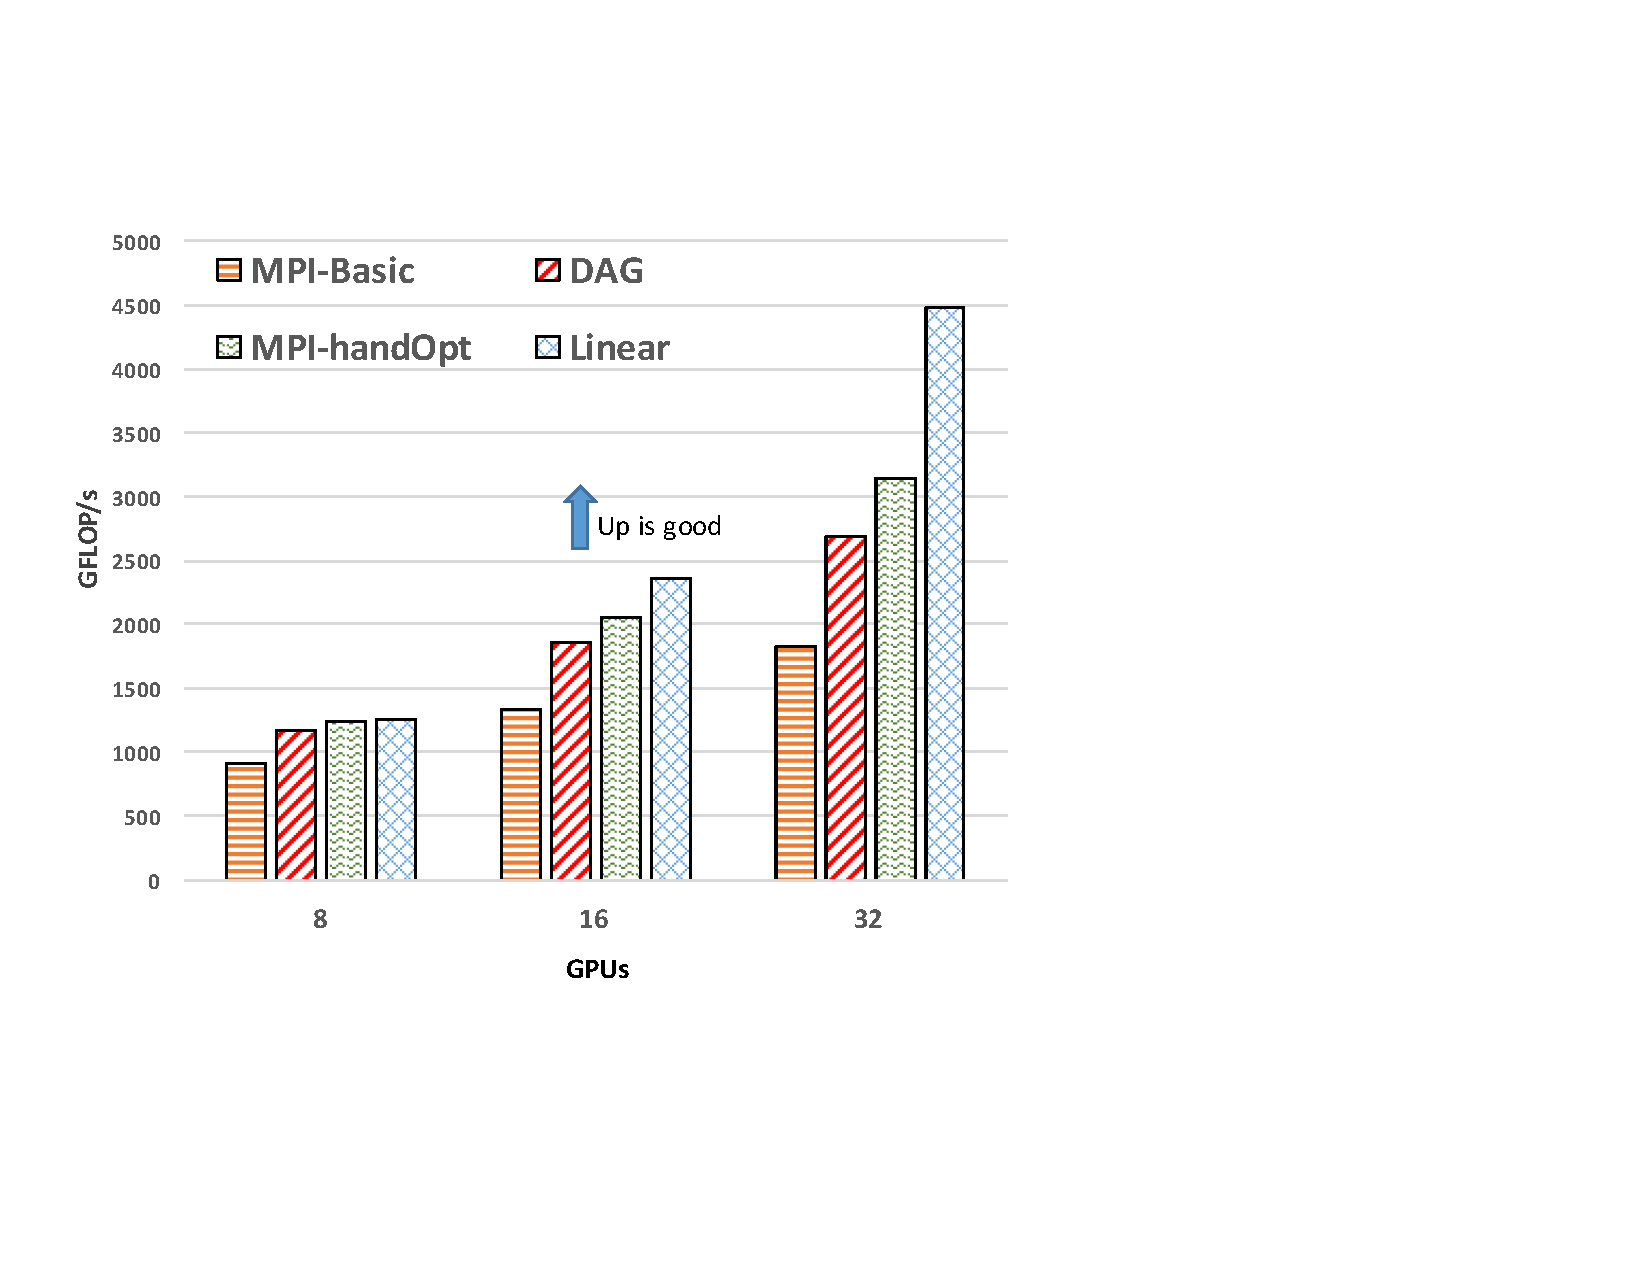
\includegraphics[width=0.49\textwidth]{figures/stencil_multiple_nodes_summit.pdf}
%\caption{Strong scaling results of 3D-Stencil on multiple nodes of SummitDev. Problem size is fixed at 1024x1024x2048.}
%\label{fig:stencil_multiple_nodes}
%\end{figure}
%

%Fig.~\ref{fig:stencil_multiple_nodes} shows the performance of all code variants.
%As expected, we observe higher impact of communication on the performance.
%In this study, we do strong scaling with 1D decomposition.
%Thus, as the number of GPUs increases the amount of communication data remains the same while the number of Flops computed on each GPU decreases.
%{\em DAG} and {\em MPI-HandOpt} can tolerate this relative increase in communication overhead via overlapping both host-host and host-GPU communication with computation.
%On 8 GPUs, these code variants meet the {\em Linear} performance.
%On 16 and 32 GPUs, although the amount of computation is not sufficient to hide all communication, the performance improvement remains significant.
%Compared to {\em MPI-HandOpt}, {\em DAG} is slightly slower.
%The performance gap can be explained by the scheduling overhead, which increases when tasks become smaller.
%In real-world scientific problems, we expect tasks to be much larger since each data element is associated with multiple physical variables. 
%Under this scenario, we expect the performance gap to be small as it is on 8 GPUs in Fig.~\ref{fig:stencil_multiple_nodes}.




%\subsubsection{Communication hiding}
%We now extend the experiment to multiple GPUs.
%In this experiment, we evaluate the benefit of hiding the communication overheads among the GPUs.
%To this end, we configure the runtime in two modes: {\em no overlap} and {\em overlap}.
%The former uses blocking CUDA memory copy routines to transfer data between host and GPUs while the latter uses non-blocking variants.
%Since the fine-grained scheduler is not compatible with blocking mode (the persistent kernel runs to completion while blocking routines cannot proceed until all previously submitted CUDA kernels have completed), we use the coarse-grained scheduling policy for both the blocking and non-blocking modes.

%Fig.~\ref{overlap} shows results of three applications under two communication modes.
%In this study, we do not replicate the input matrices of the 2.5D Cannon's algorithm because the communication avoiding technique may interfere with the communication overlap.
%We will study this interference later in Sec~\ref{subsec:CAvsOlap}.
%It can be seen in Fig.~\ref{overlap} that on three applications {\em overlap} always outperforms {\em no overlap}.
%In Cholesky, we place data on the host and stream them to GPUs to perform the compute-intensive {\em update} kernel.
%Thus, even on one GPU, communication arises.
%\footnote{Although we do not show results of 2.5D Cannon and 3D Stencil on one GPU, it's worth noting that computing on one GPU does not incur communication cost since we initially place data on the GPU.
%As a result, we do not observe performance improvement when running these two applications on only one GPU.}
%On multiple GPUs, we realize notable performance improvement via overlapping communcation with computation.
%The overall time reduction is 10\% more or less.
%For Stencil, however, we see a higher speedup (up to 1.85$\times$) due to the following reason.
%At a small scale 1D decomposition works best since it does not require the costly packing and unpacking operations.
%However, with a 1D decomposition scheme the amount of communication does not decrease as the number of GPUs increases.
%Thus, the more GPUs the higher communication relative to computation, resulting in a better improvement due to overlap.
%Unlike 3D Stencil, experiments on the other two applications use a 2D decomposition scheme.
%Thus, the communication over computation ratio does not change much as the number of GPU increases.

%\begin{figure*}[htb]
%\centering
%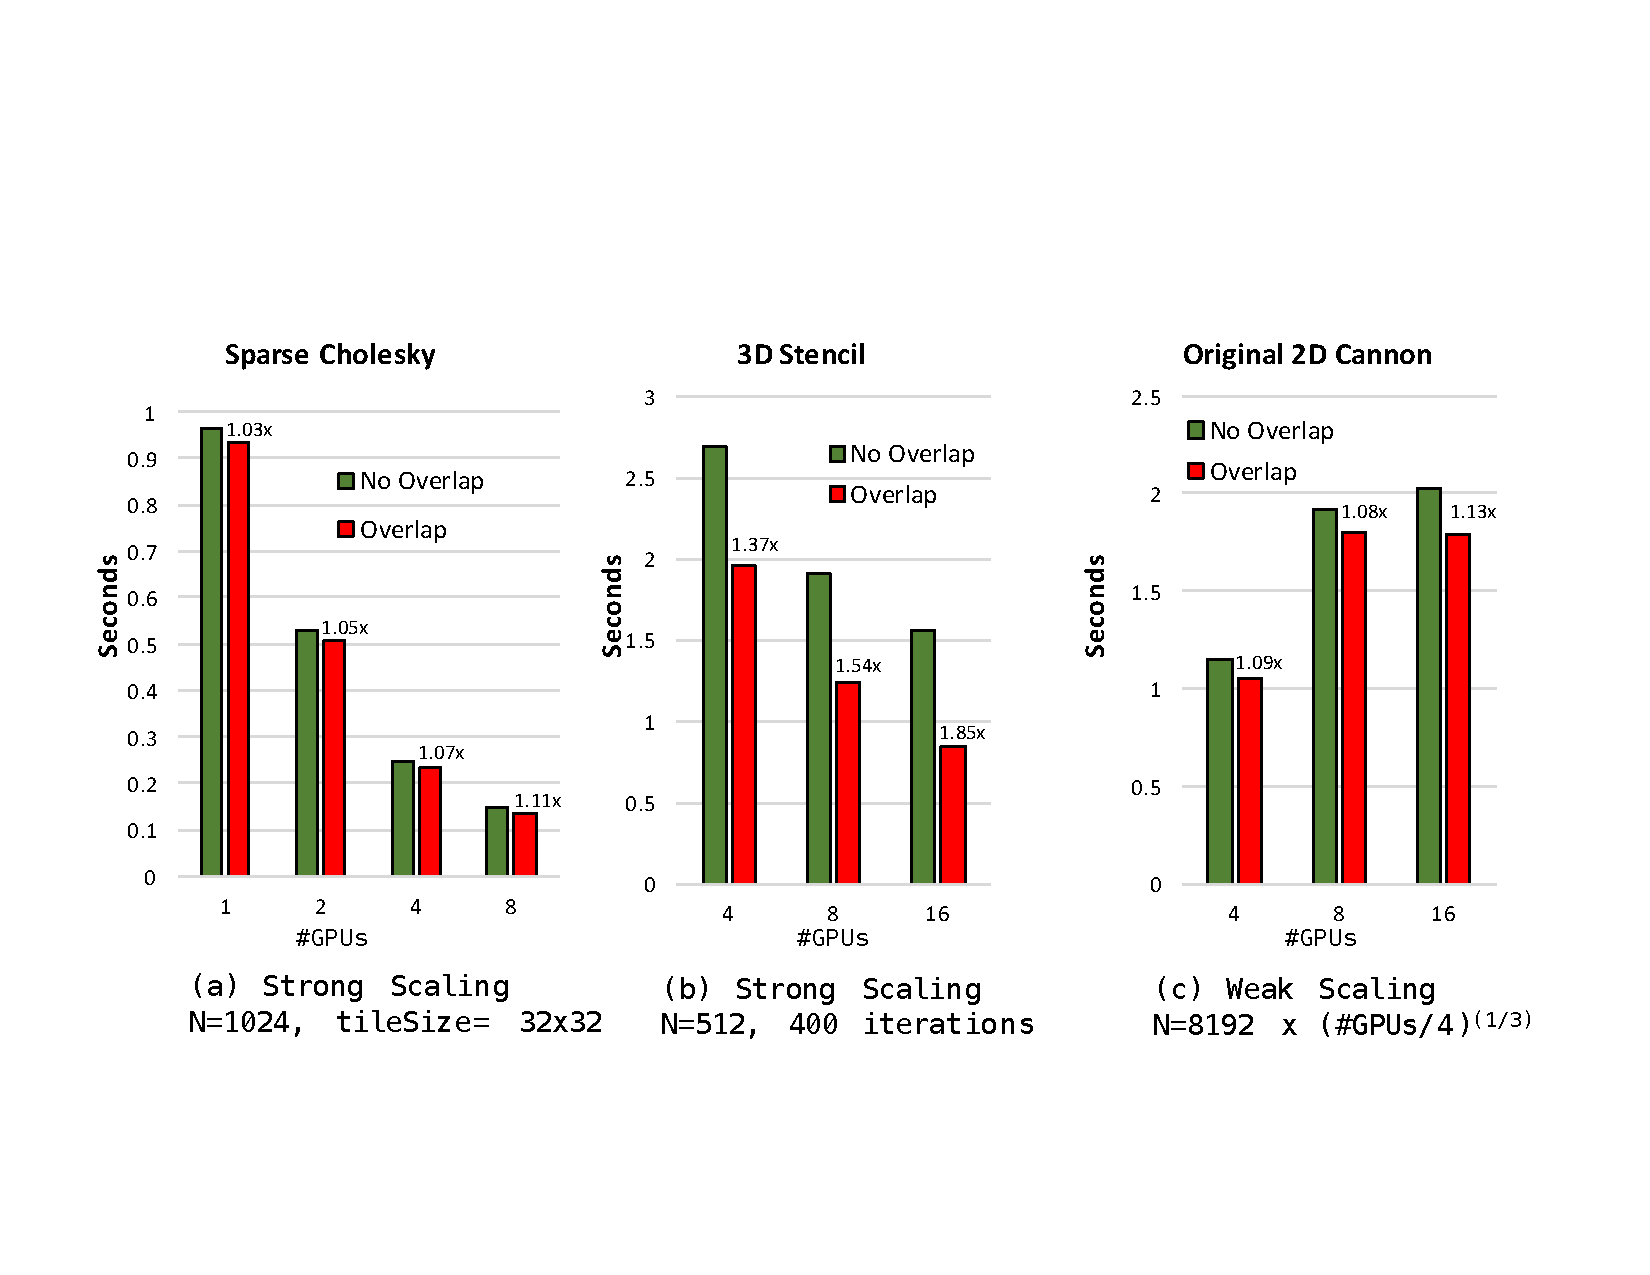
\includegraphics[width=0.9\textwidth]{figures/overlap.pdf}
%\caption{Hiding communication automatically via overlap
%\samW{How much potential was there for overlap in the first place?}
%%\samW{When strong scaling, there is a region where it might be viable.}
%\samW{When weak scaling, you may always be outside the range where overlap is viable.}
%}
%\label{overlap}
%\end{figure*}

%\begin{figure}[htb]
%\centering
%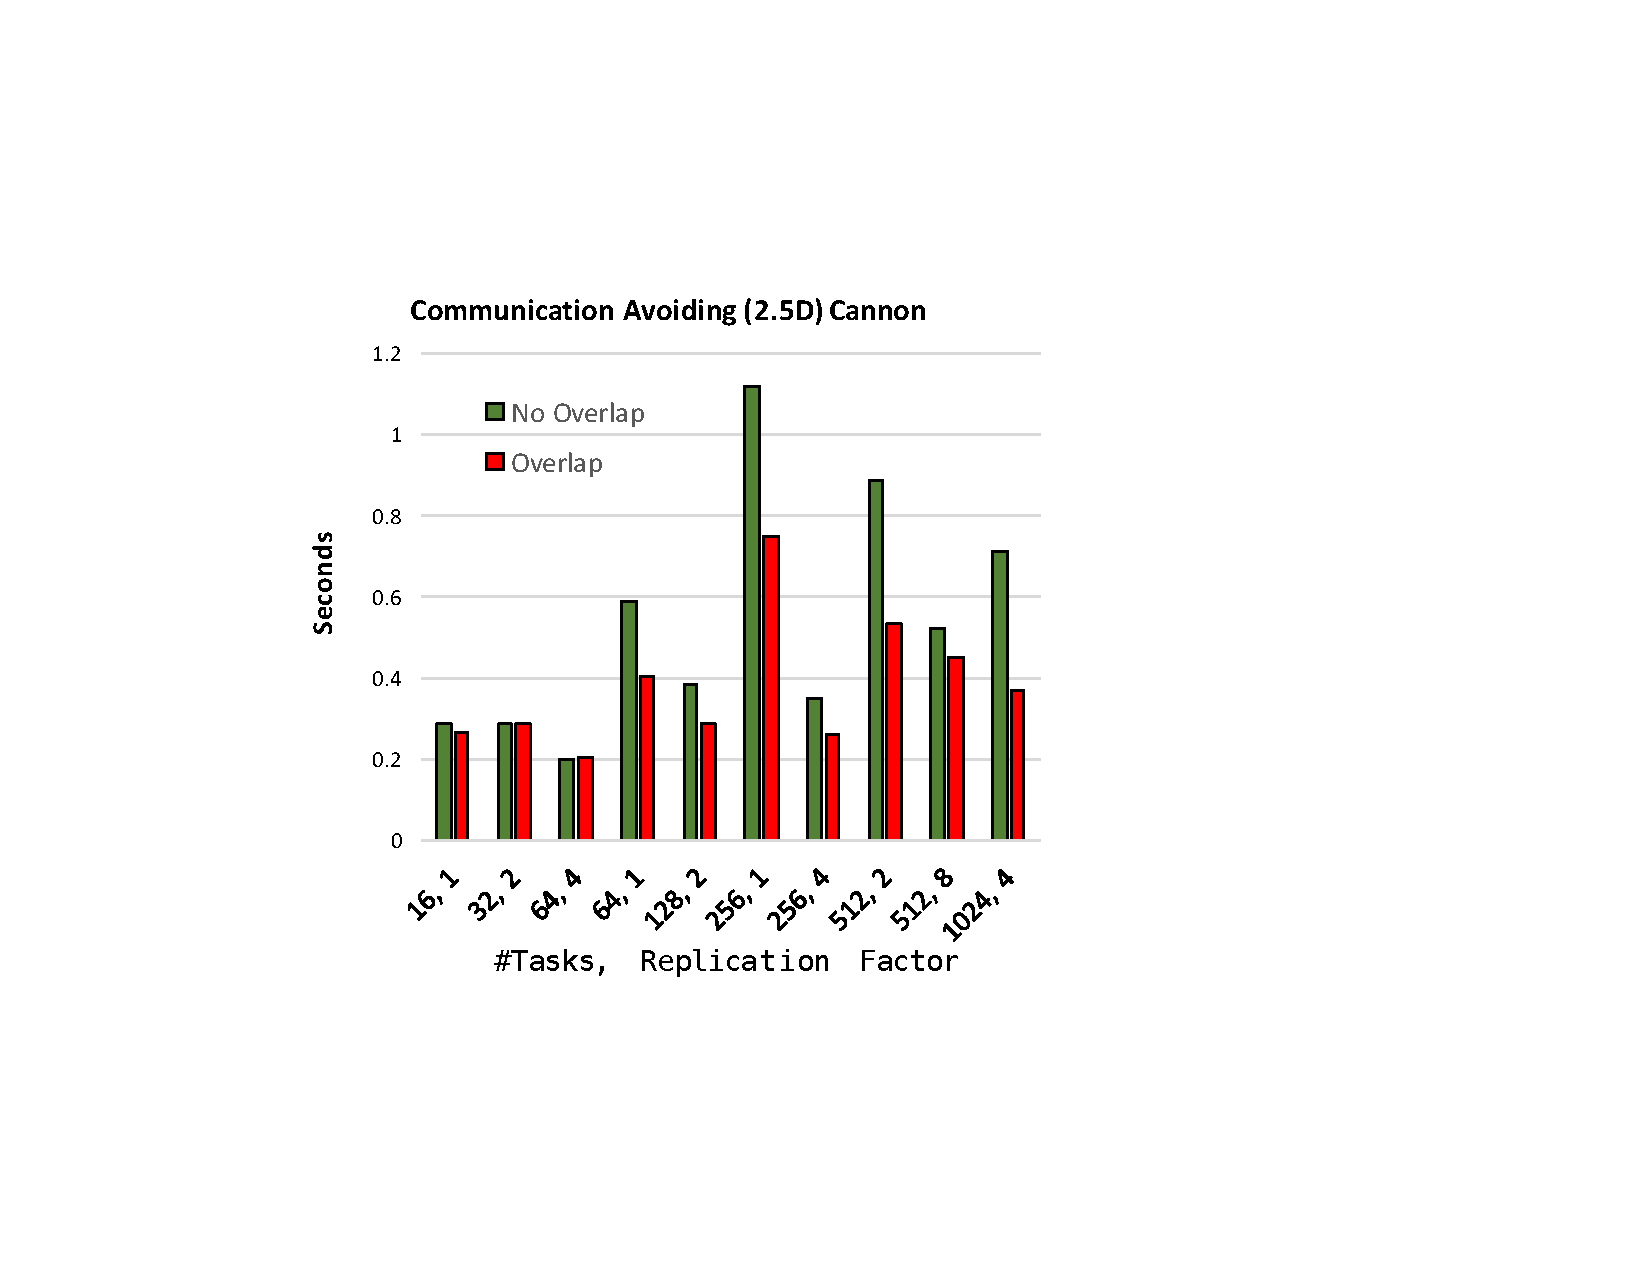
\includegraphics[width=0.49\textwidth]{figures/CA_4096.pdf}
%\caption{2.5D Cannon on 16 GPUs using small matrices (N=4096). The communication avoiding technique results in many task configurations. For good configurations (e.g. \{64, 4\}), there is not much room for the communication overlap. However, for poor configurations (e.g. \{1024, 4\}) the overlap technique does a good job in further increasing the performance}
%\label{CA_4096}
%\end{figure}

%\subsubsection{Interference between communication avoiding and hiding}
%\label{subsec:CAvsOlap}
%Now let's study the behavior of {\em overlap} when the communication avoiding technique is enabled.
%Fig.~\ref{CA_4096} shows the run time of the 2.5D Cannon program when performing matrix multiplication on 16 GPUs.
%We can see that replicating matrices substantially reduces the run time.
%Notable examples are  \{64, 4\} compared to \{64, 1\} and \{256, 4\} compared to \{256, 1\}.
%If most of the data communication can be avoided, there is not much left to hide.
%However, the number of these optimal replication configurations is very small compared to the combination of task and replication spaces.
%As a result, the programmer may need to brute force many potential configurations to find the best one.
%This requirement is costly and time consuming.
%Luckily the overlapping technique can work with communication avoiding within the same application.
%Thus, if the programmer does not pick the best replication configuration, he/she can rely on the communication overlap to realize comparable performance.
%For example, the {\em overlap} performance on configurations \{128, 2\}, \{256, 4\}, or the most wanted \{64, 1\} is  acceptable. 
%We can see that there are many of such configurations, allowing the programmer to guess one easily.



\section{Related work}
\label{sec:related}
The benefit of using a task-based execution model on traditional multi-core processors has been recognized by the HPC community for years, e.g. Cilk/Cilk++~\cite{cilk,BlumofeJoKu95}, Charm/Charm++~\cite{charm++}, Bamboo~\cite{bamboo}, DPLASMA\cite{dplasma}, OMPSs~\cite{ompss}, and Habanero-C MPI~\cite{Chatterjee:2013:HCMPI}.
However, the question of whether a task dependency graph program with many fine-grained tasks can run efficiently on an accelerator (e.g. GPU) has not yet been thoroughly answered.
As a result, many current runtimes for GPUs schedule each single task on the whole GPU (e.g. Legion~\cite{legion} and CNC-HC~\cite{cnc-hc}).
As the number of cores per accelerator increases quickly, this limitation puts the programmer under the pressure of optimizing their kernels so they can scale linearly as the accelerator architecture evolves.

Recently more research has been focusing on launching a CUDA kernel on a portion of the GPU.
In~\cite{fillNRetreat}, Wu et al. presented a technique called {\em fill and retreat}, which allows a CUDA kernel to run on a group of selected SMs.
With this technique the programmer can efficiently bundle multiple CUDA kernels to run on a single GPU at a time.
Abdelfattah et al. also used a similar technique to batch small CUDA kernels in a Cholesky factorization program in order to improve the throughput~\cite{batchedCholesky}.
Our solution relies on a task scheduler to factor the scheduling policy out of the application program.
As a result, the programmer can take the benefit of fine-grained scheduling at a very small amount of programming cost.

%Multi-GPU programming is also an important support because the memory capacity of each individual GPU is very limited.
%There are MPI implementations that provide this support, e.g. MPI-ACC~\cite{mpiacc, mpiacc1} and Mvapich~\cite{mvapich2gpu}.
%However, with these tools the programmer has to explicitly move data.
%We provide a dataflow programming model that supports distributed-memory architectures, allowing the runtime to move data across memory address spaces transparently.
%In addition, the data movement is non-blocking and independent of computations, overlapping communication with computation.

%Our runtime is general-purpose.
%Thus, it supports a wide range of applications, as opposed to other domain-specific runtimes such as MAGMA~\cite{MAGMA}, Physics~\cite{physics}, and Patus~\cite{patus}.


\section{Conclusion}
\label{sec:conclusion}
We have presented a task-based programming model and runtime system for accelerator-based clusters.
Experimental results show that with the new code representation the programmer can realize better performance.
Our solution offers a simple interface so the programmer can realize performance benefits without the needs of redesigning the algorithm and aggressively restructuring the source code as the system architecture evolves.
We deem that our paper not only has impact on application development, but it can also initiate further research on HPC libraries such as developing and tuning cuSPARSE routines for running on the same GPUs. 


\section*{Acknowledgments}
This material is based upon work supported by the Advanced Scientific Computing Research Program in the U.S. Department of Energy, Office of Science, under  Award Number DE-AC02-05CH11231.
RambutanAcc and application codes were developed on TiDA, a workstation housed at LBNL, with GPUs provided by NVIDIA.
We would like to thank Paul Hargrove for his great help on GASNet.

%\input{artifact}

\bibliographystyle{splncs03}
\bibliography{ref} 


\end{document}
